% Chapter Template

\chapter{Frontiers in \emph{Quantum chaology}} % Main chapter title

\label{Chapter6} % Change X to a consecutive number; for referencing this chapter elsewhere, use \ref{ChapterX}
\thispagestyle{empty}

\section{Numerical simulations}

The difficulties of even just approaching \QUE conjecture by Rudnick and Sarnak, for example, led researches in this area to, at least, find numerical evidence for it. In this sense, a major contribution arrived from Alex Barnett, who worked in the past ten years frequently with Peter Sarnak. He developed numerical methods for investing spectral properties of quantum system derived from billiards and his most notable project was the simulation of $\simeq30000$ eigenfunctions of the Barnett billiard (and for this reason Sarnak gave his name to this kind of billiard). In particular, this project produced evidence that \QUE holds in this case. Barnett studied the rate of equidistribution of Laplacian eigenfunctions (with Dirichlet boundary condition) by analyzing the diagonals element of the \emph{matrix coefficient} (see section \ref{subsec:mixing}) $\pscl{A\vphi_{m}}{\vphi_{n}}$, where $A$ is a suitable test $\PDO$ and $\vphi_{n}$ are eigenfunctions of eigenvalues $\lambda_{n}$.


\begin{figure}[H]
\centering
    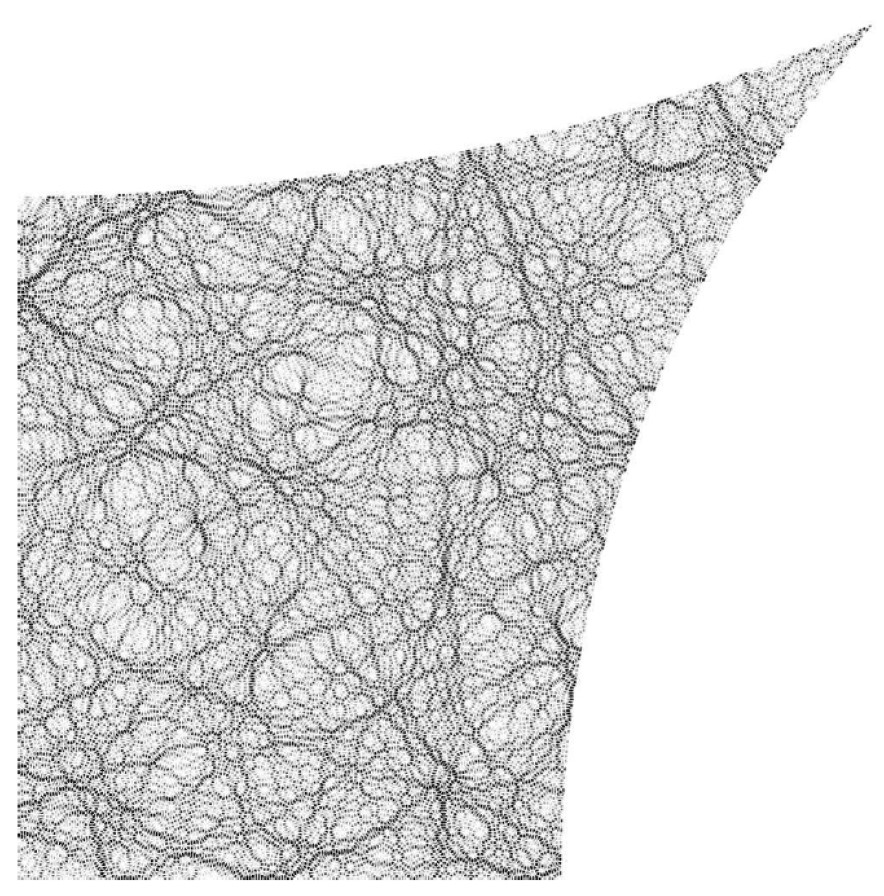
\includegraphics[scale=0.3,angle=0]{Barnett_eig_sim.jpg}
    %\caption{Variabili $X_{n}$}
  %
  \noindent\\
  \decoRule
  \caption{The density eigenfunction $\abs{\vphi_{n}}^{2}$ for $n\simeq5\times10^{4}$ and the corrispondent $\lambda_{n}\simeq10^{6}$. Computed by Alex Barnett.}
  \label{fig:barnett_eigenfunction}
\end{figure}


Barnett examinated these quantities up to $n,m\simeq 7\times10^{5}$, getting a $10^{2}$ improvement of eigenvalue magnitude over the state of art. Moreover, he developed a free \textsc{MatLab} tool to plot efficently eigenfunctions on complex domains (\textsc{mpspack}, see \url{https://github.com/ahbarnett/mpspack}).\\

Another essential support to this field, mainly about Maass forms and quantum chaos problems relative to the modular group and its subgroups arrived, starting from the work of \cite{Hejhal:triang}, recently from Friderik Stromberg (\cite{Stromb:article}), who succeded in calculating the first $10.000$ eigenvalues for $X(1)$. Moreover, Holger Then, with the joint work of already mentioned Barnett, managed to compute and plot eigenfunctions with an high accurancy (\cite{Barnett:asym_rate},\cite{Then:article}).



\begin{figure}[H]
\centering

    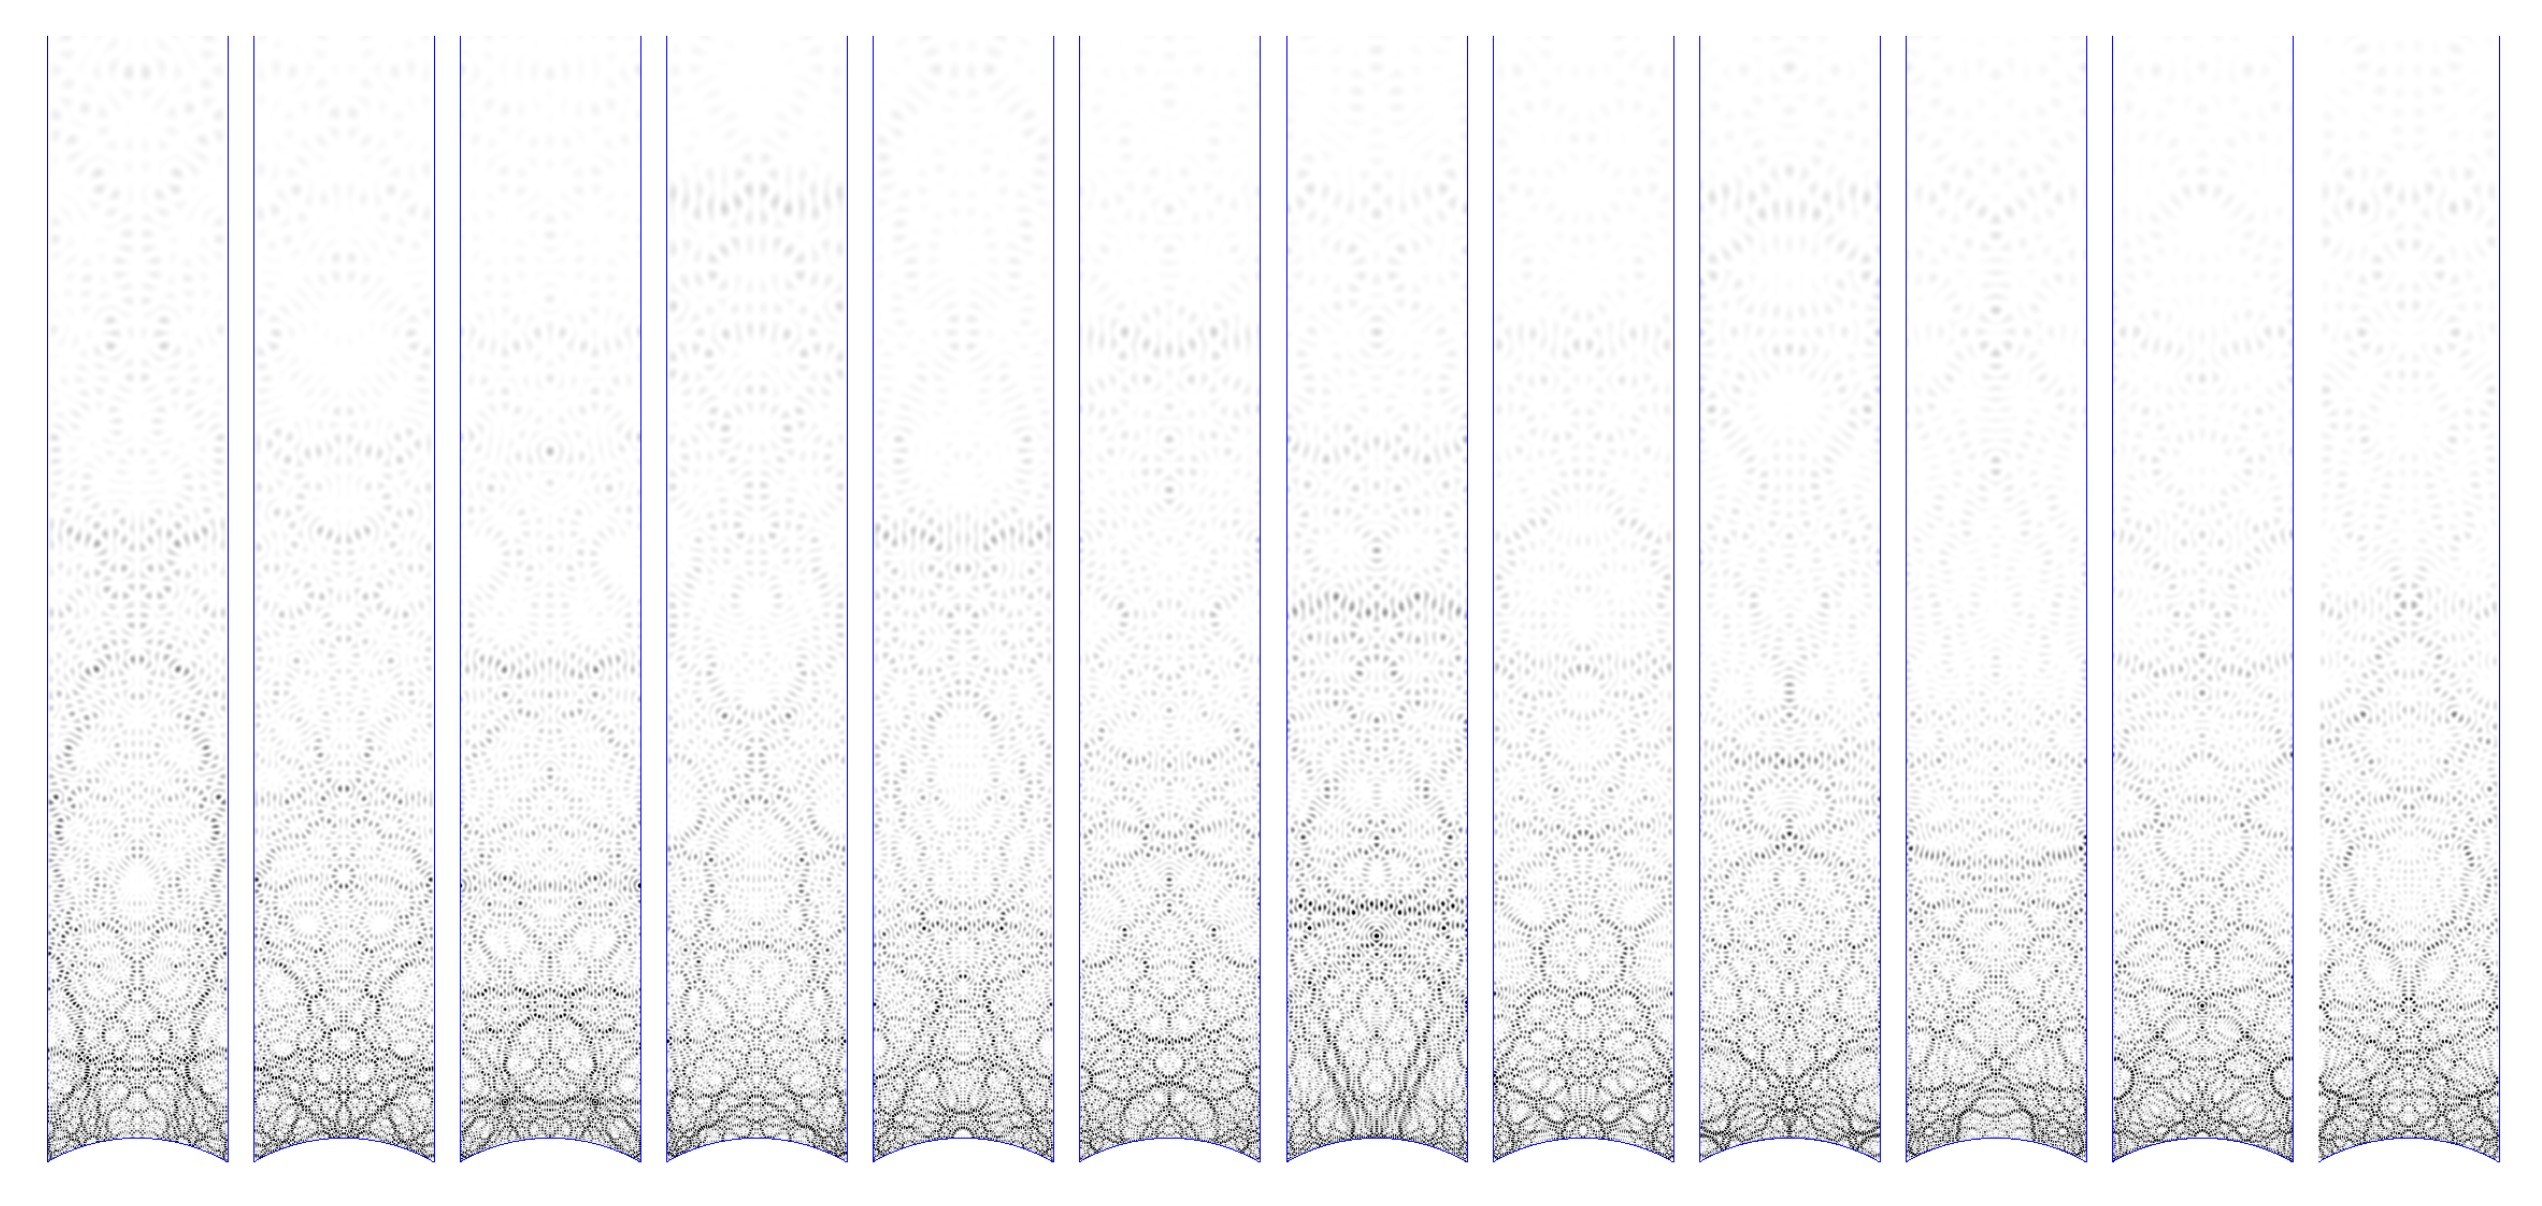
\includegraphics[scale=0.3,angle=0]{mod_surface_then.jpg}
    %\caption{Variabili $X_{n}$}

  %
  \noindent\\

  \decoRule
  \caption{12 consecutive Maass forms (5600th eigenvalue and so on), i.e. laplacian eigenfunctions on the modular surface, computed by Holger Then and Alex Barnett}
  \label{fig:holg_then_eig_modul}
\end{figure}







Not to forget is the breakthroughing contributions due to Strohmaier and Uski, who computed with very high accurancy, the first $1000$ eigenvalues of Laplacian on Bolza surface, using a different algorithm described in \cite{Stroh:comput} best suited for compact surfaces of genus $2,3,4$ (thus very different cases from the modular surface).


\begin{figure}[H]
\centering
  \begin{subfigure}[b]{0.2\textwidth}
  \centering
    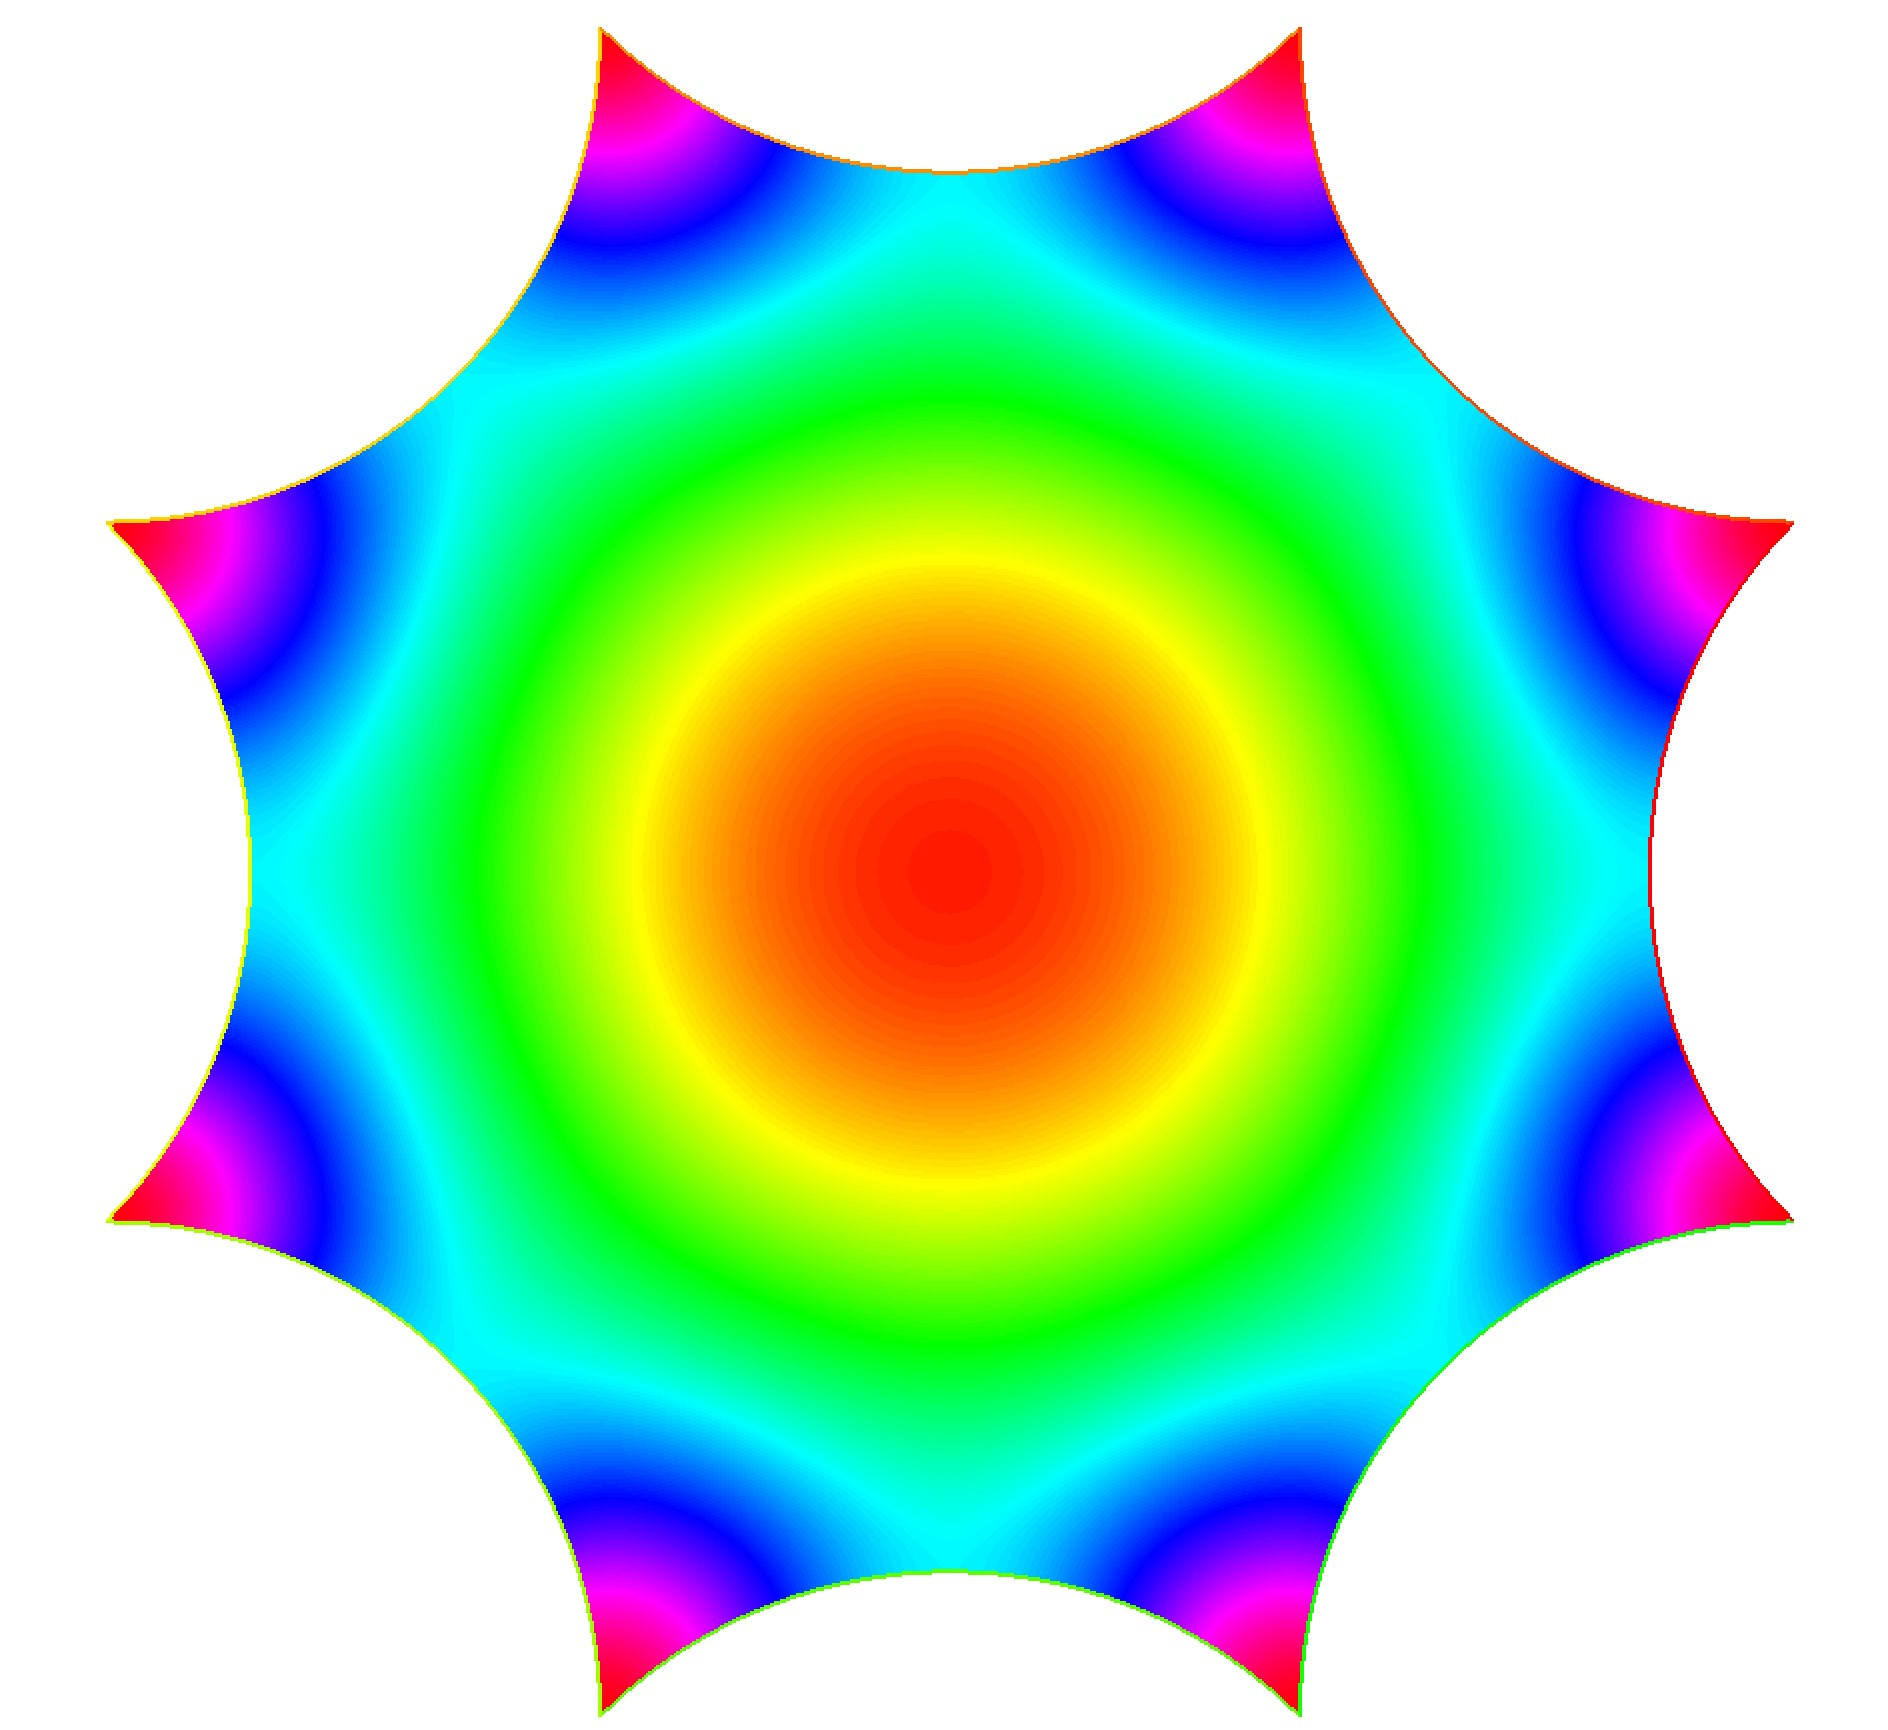
\includegraphics[scale=0.1,angle=0]{bolza1.jpg}
    %\caption{Variabili $X_{n}$}
    \label{fig:eig_bolza1}
  \end{subfigure}
  %
  \noindent\\
  \begin{subfigure}[b]{0.2\textwidth}
  \centering
    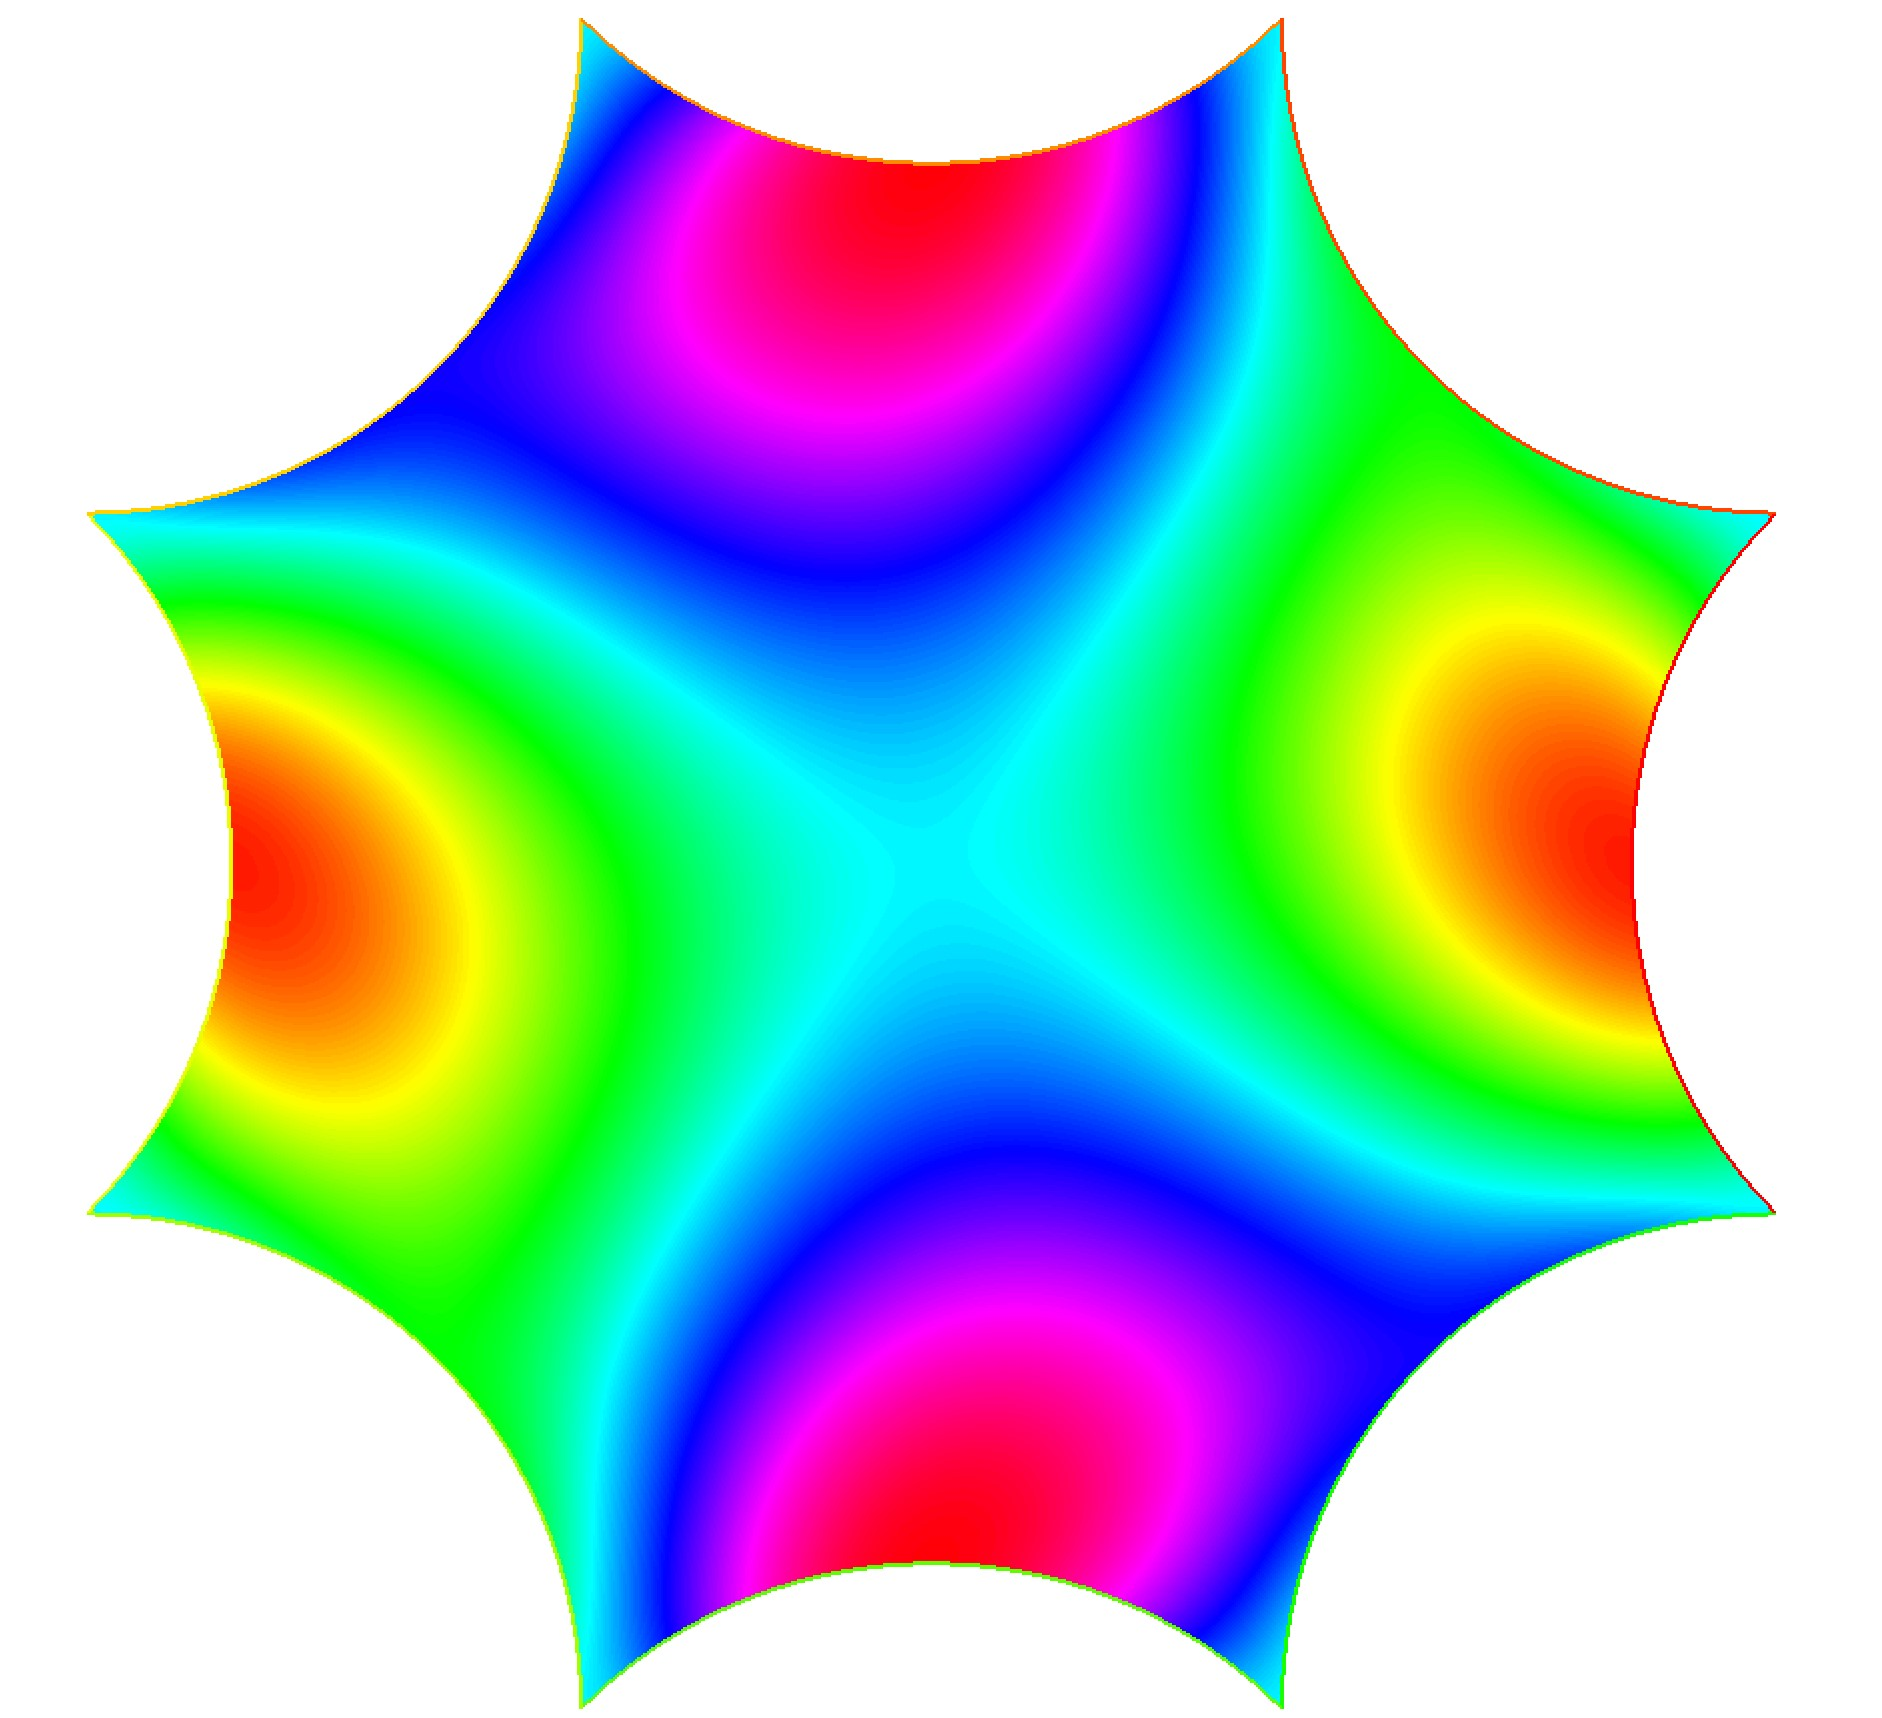
\includegraphics[scale=0.1,angle=0]{bolza2.jpg}
    %\caption{Variabili $X_{n}$}
    \label{fig:eig_bolza2}
  \end{subfigure}
  \begin{subfigure}[b]{0.2\textwidth}
  \centering
    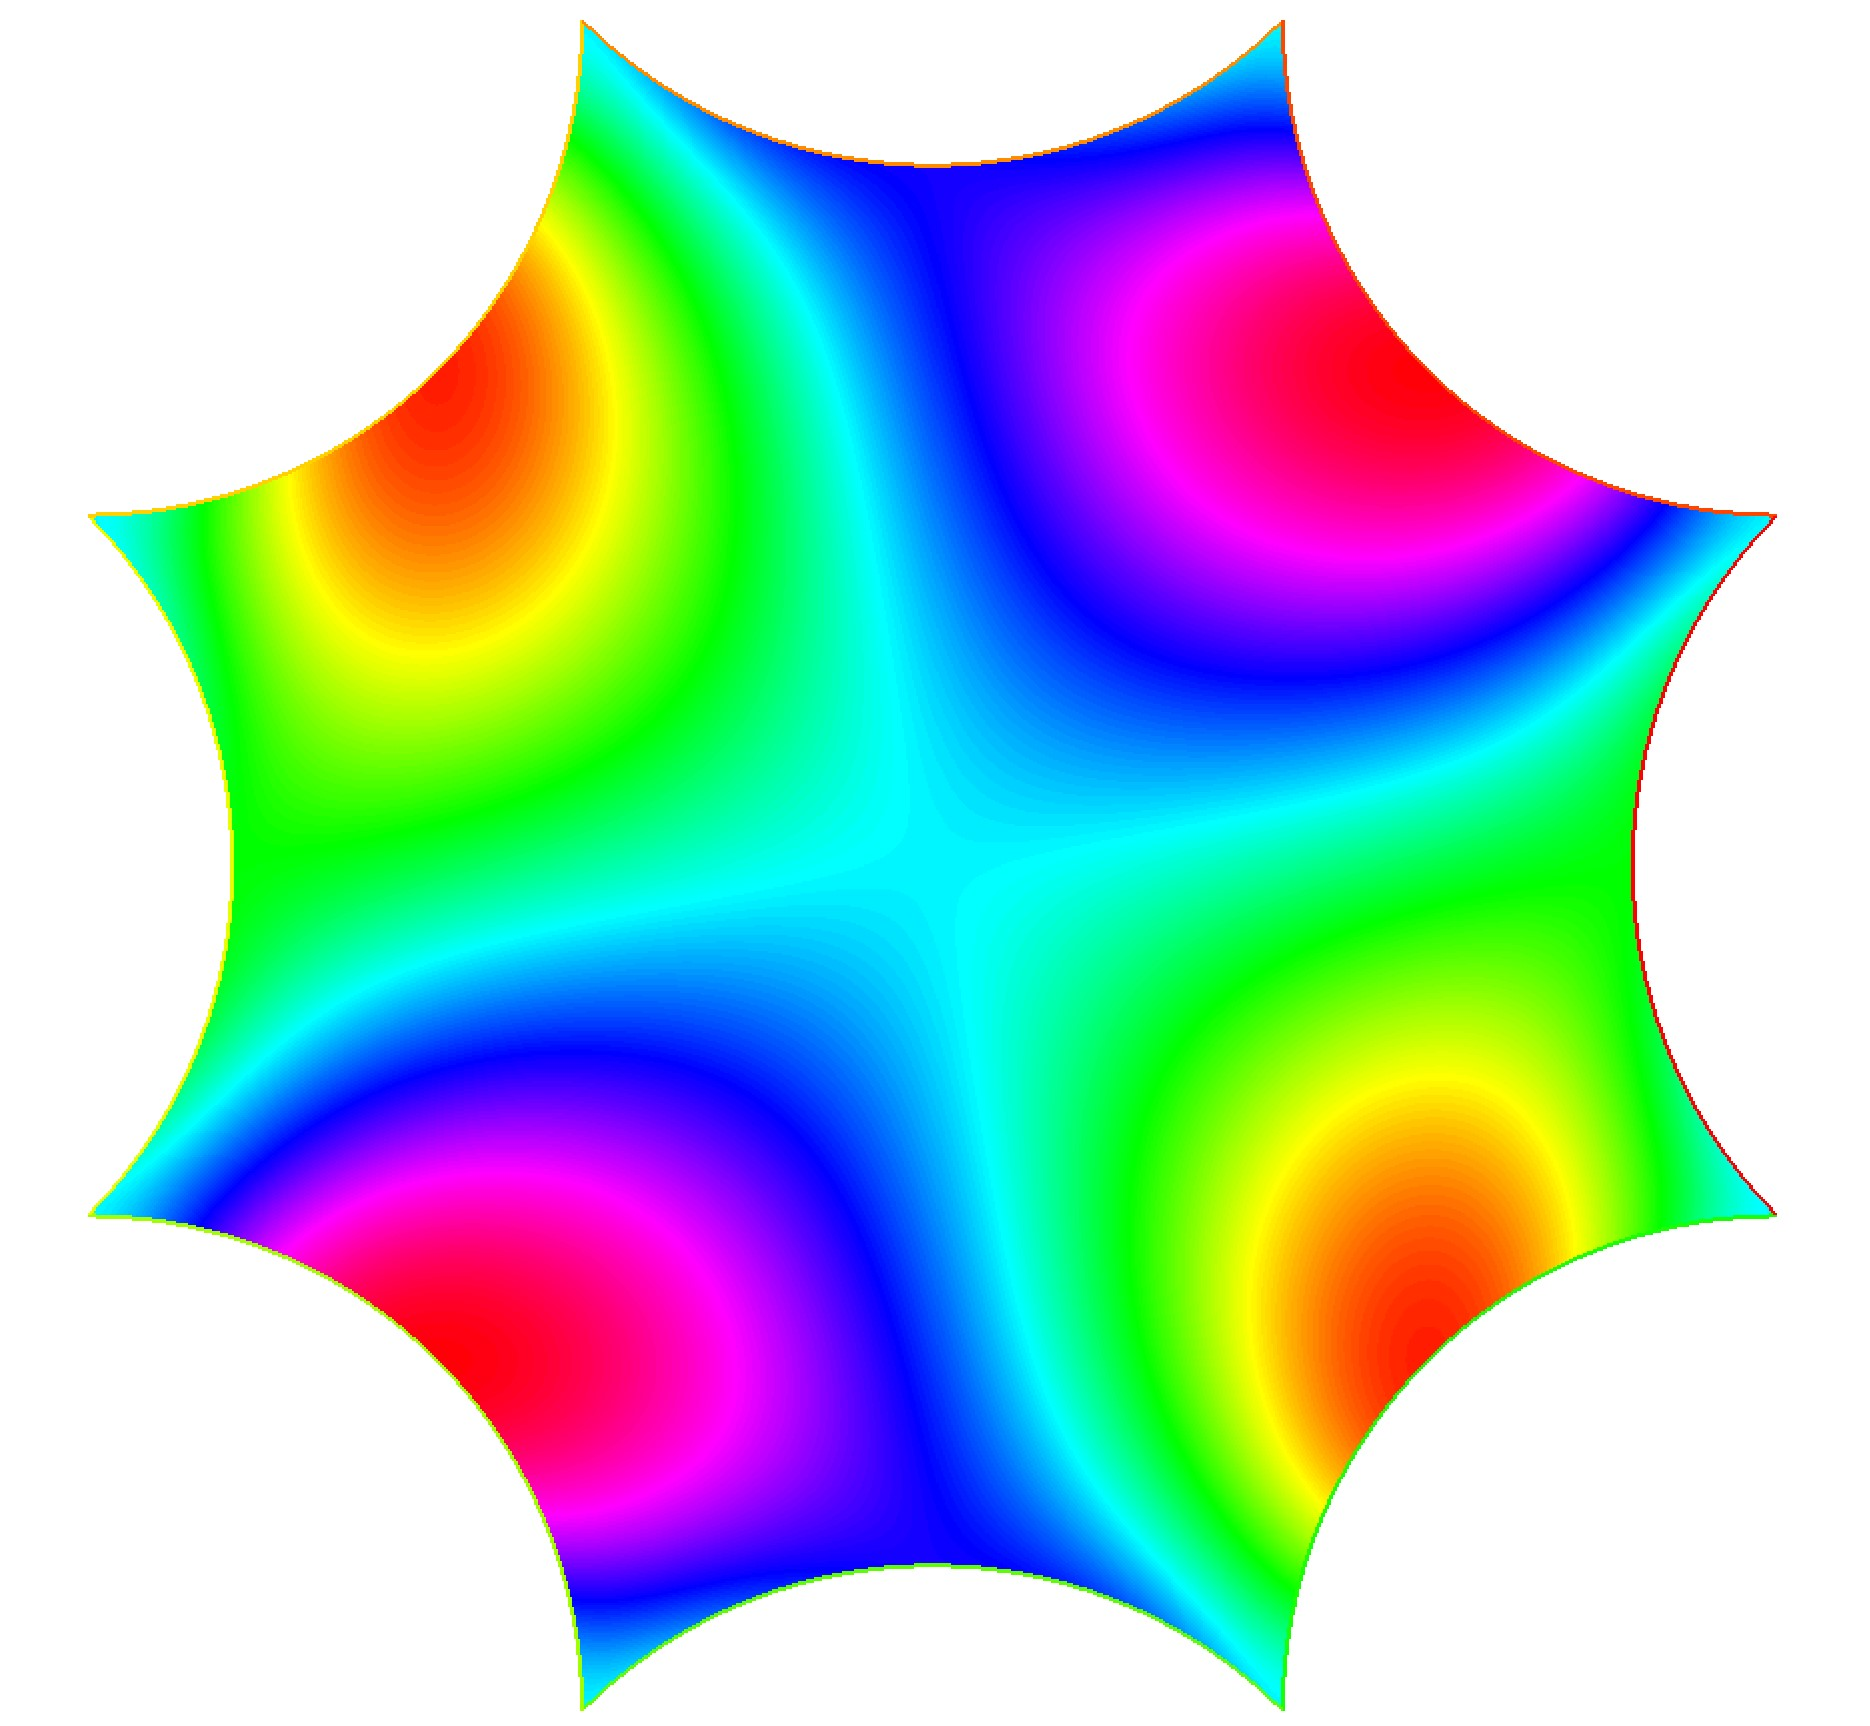
\includegraphics[scale=0.1,angle=0]{bolza3.jpg}
    %\caption{Variabili $X_{n}$}
    \label{fig:eig_bolza3}
  \end{subfigure}
  \noindent\\
  \decoRule
  \caption{The three eigenfunctions on Bolza surface, corrisponding to the first eigenvalue $\lambda=3.8388872\ldots$. See \cite{Stroh:comput}}
  \label{fig:first_3_bolza_eig}
\end{figure}



\begin{figure}[H]
\centering
  \begin{subfigure}[b]{0.2\textwidth}
  \centering
    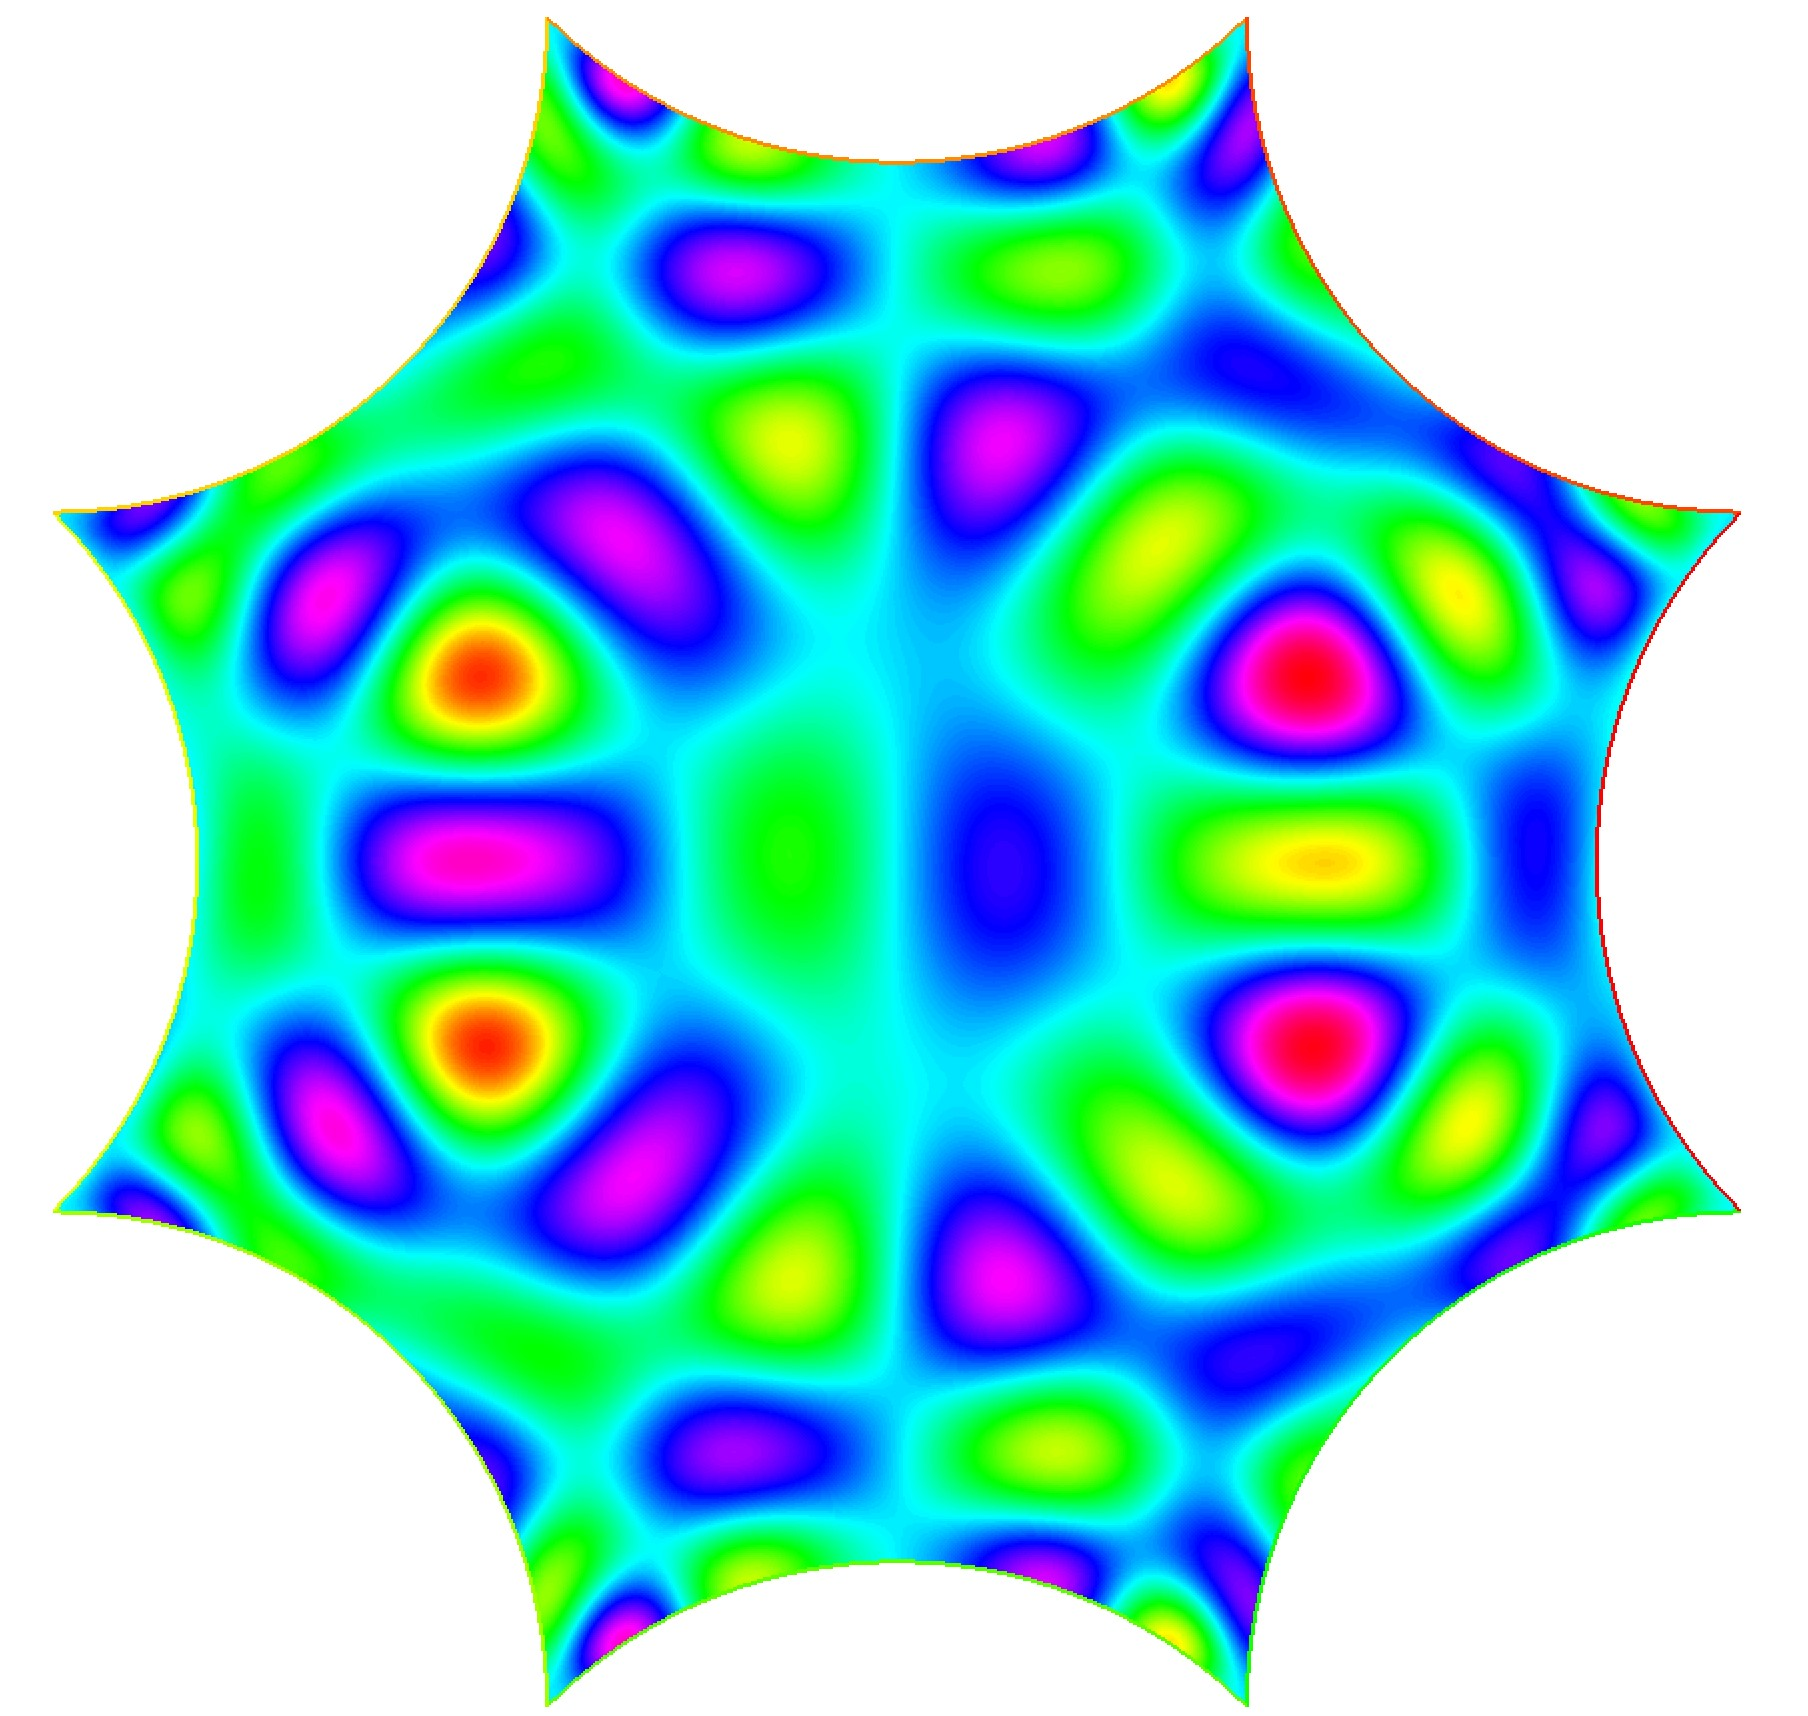
\includegraphics[scale=0.08,angle=0]{bolza5.jpg}
    %\caption{Variabili $X_{n}$}
    \label{fig:eig_bolza4}
  \end{subfigure}
  %
  \begin{subfigure}[b]{0.2\textwidth}
  \centering
    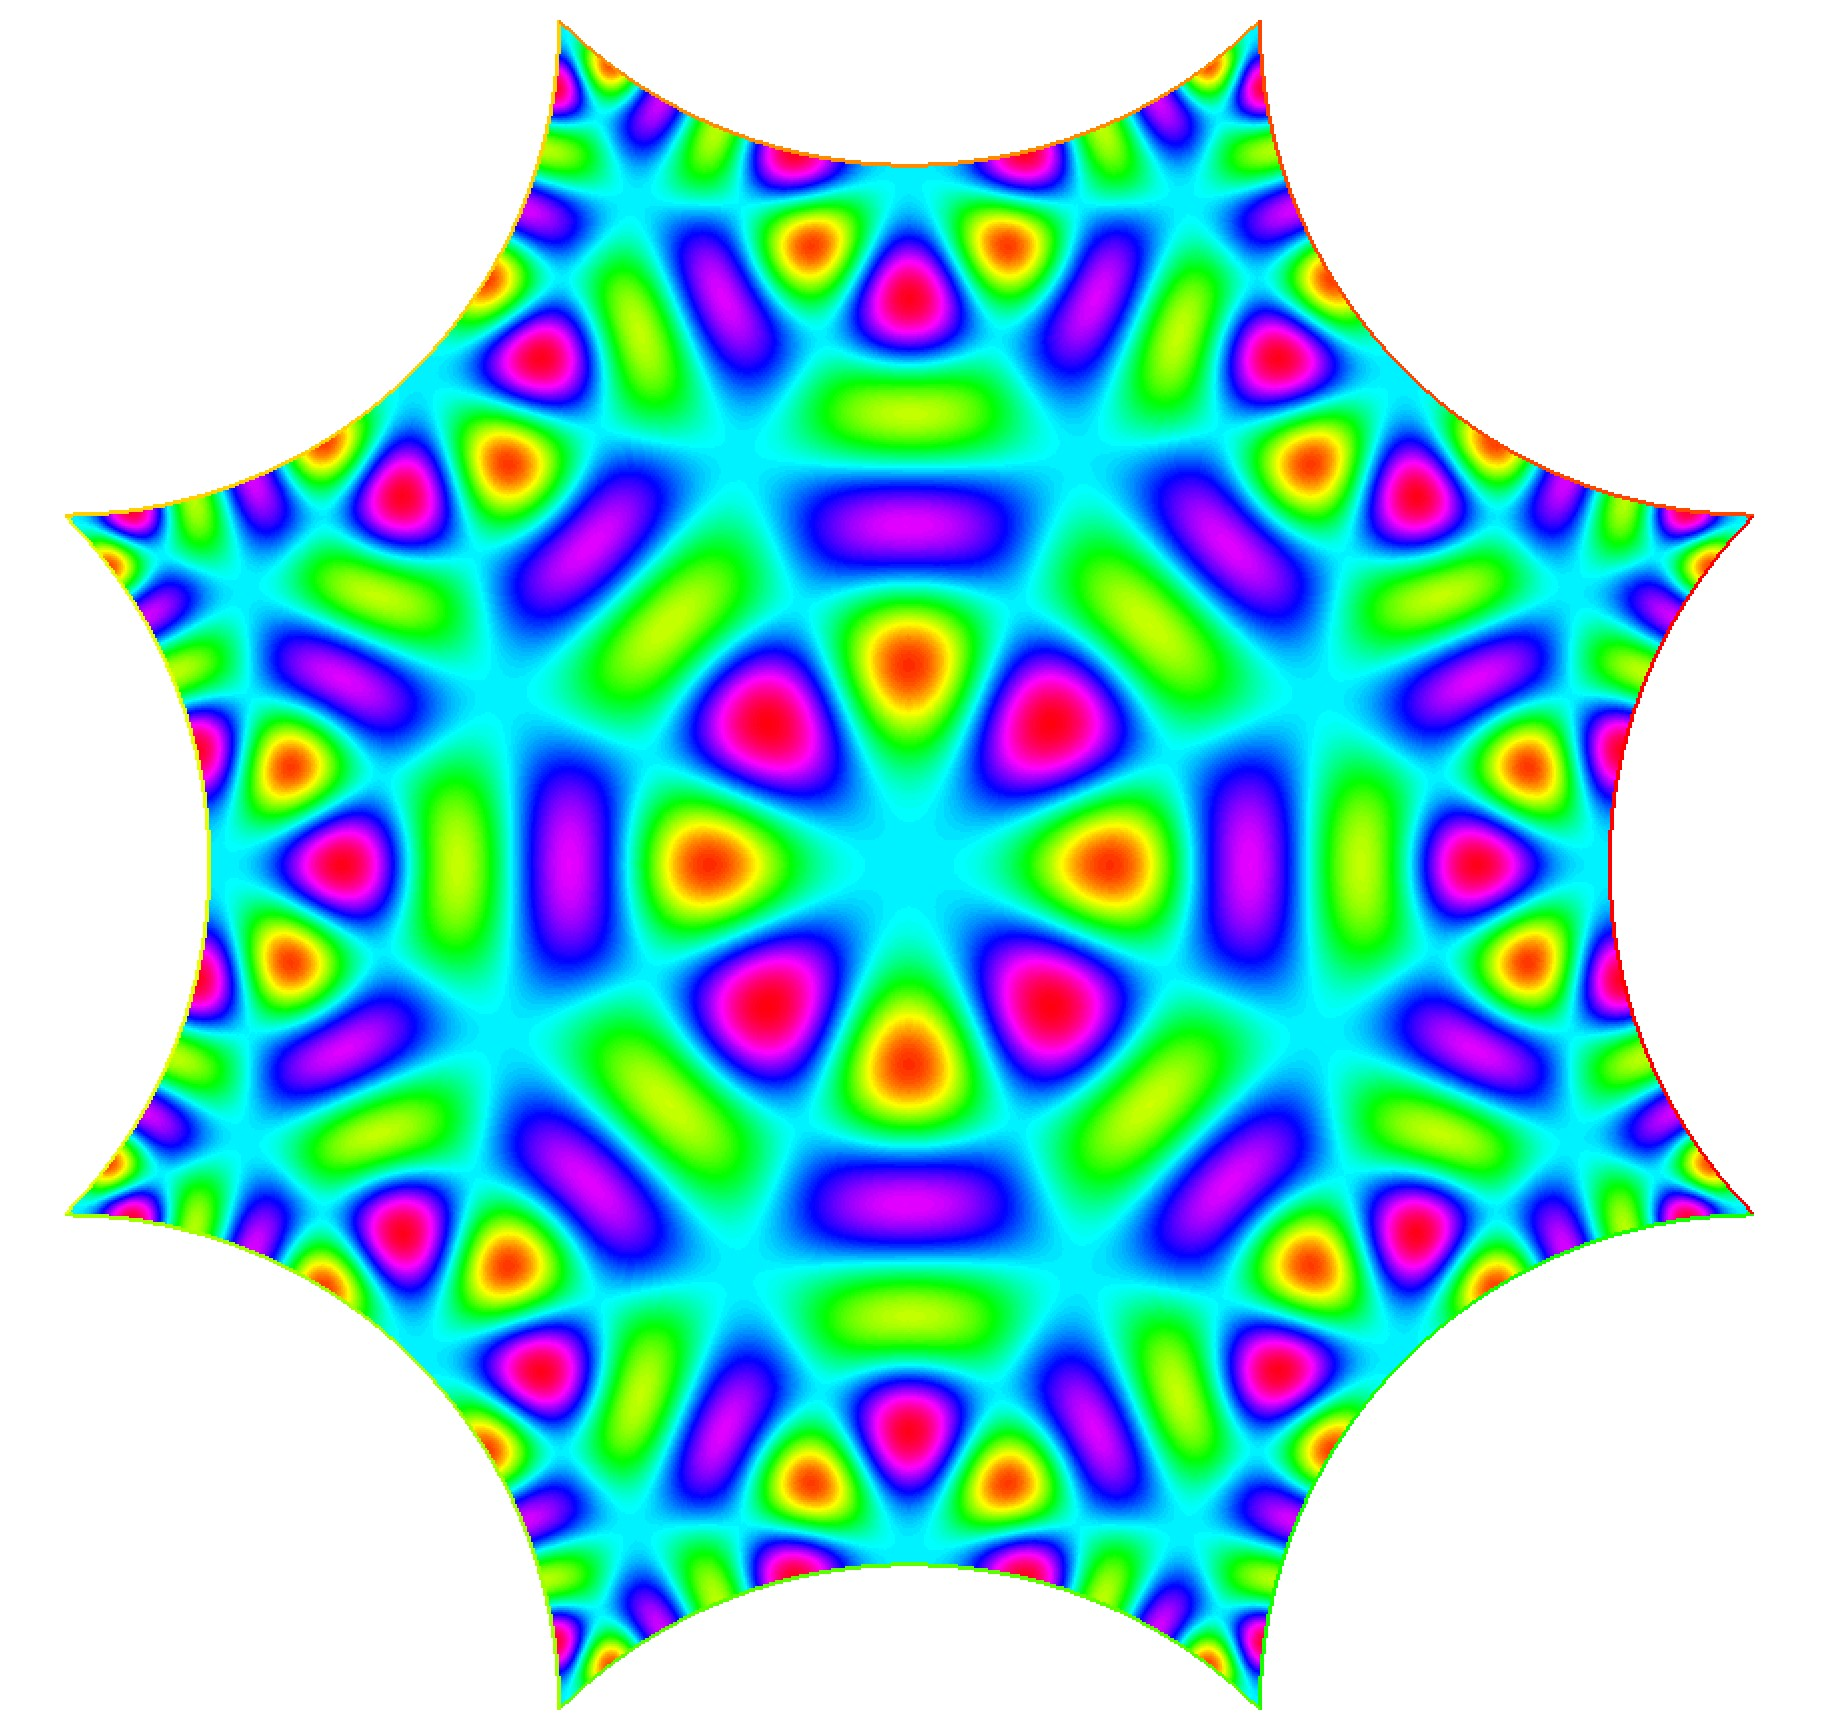
\includegraphics[scale=0.08,angle=0]{bolza6.jpg}
    %\caption{Variabili $X_{n}$}
    \label{fig:eig_bolza5}
  \end{subfigure}
  \begin{subfigure}[b]{0.2\textwidth}
  \centering
    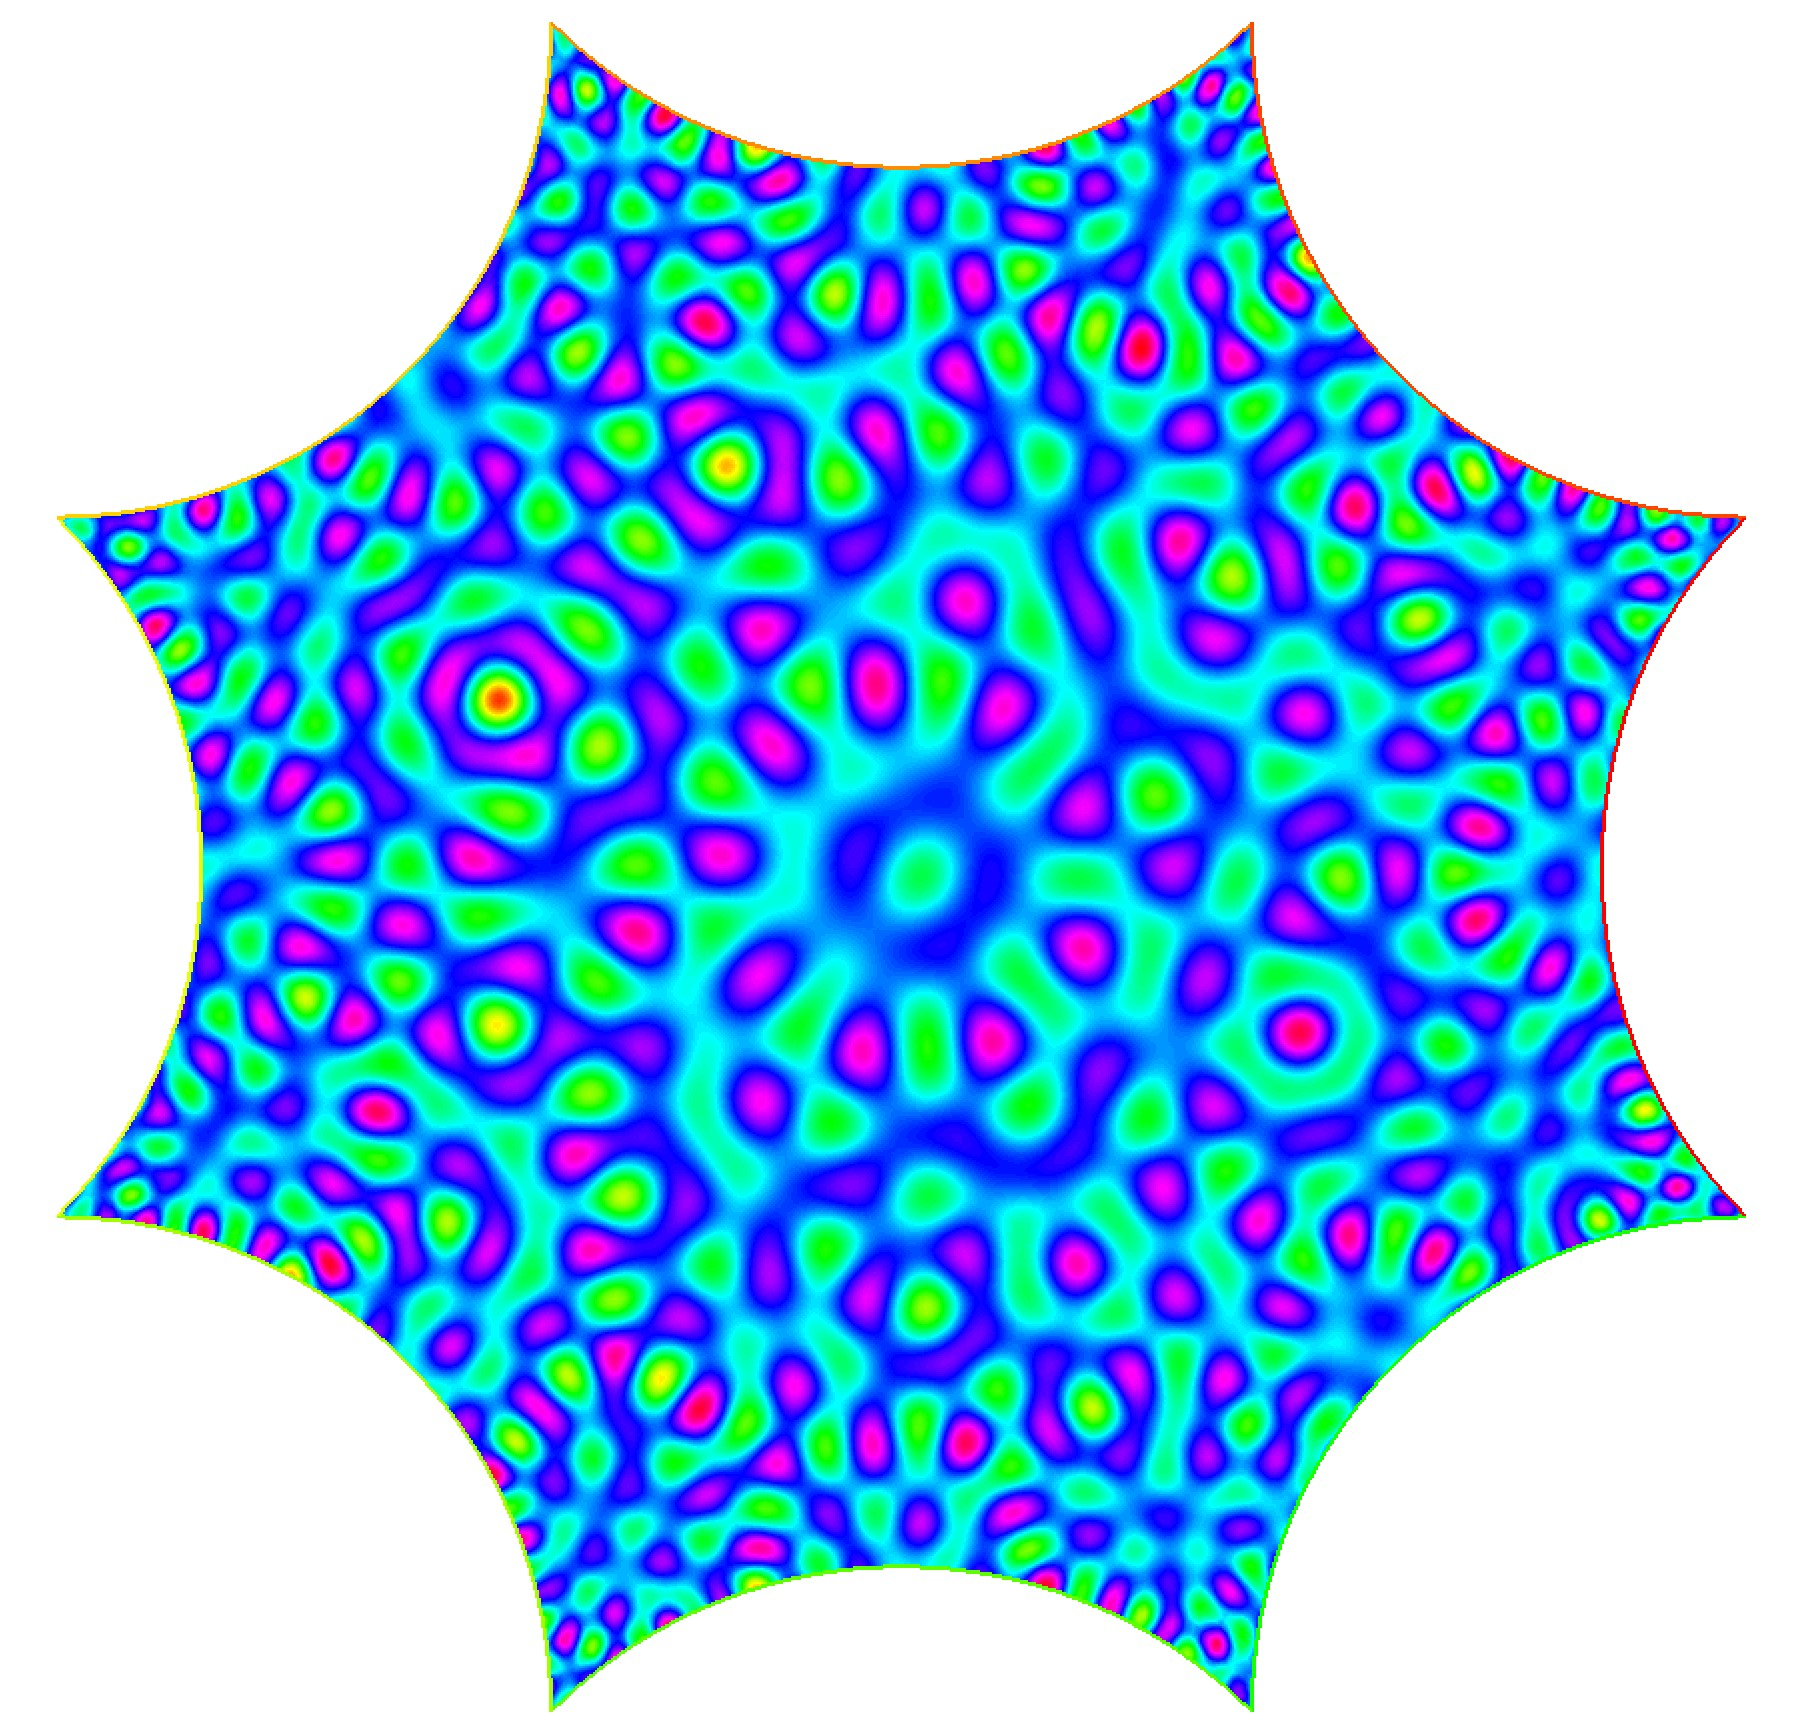
\includegraphics[scale=0.08,angle=0]{bolza7.jpg}
    %\caption{Variabili $X_{n}$}
    \label{fig:eig_bolza6}
  \end{subfigure}
    \begin{subfigure}[b]{0.2\textwidth}
  \centering
    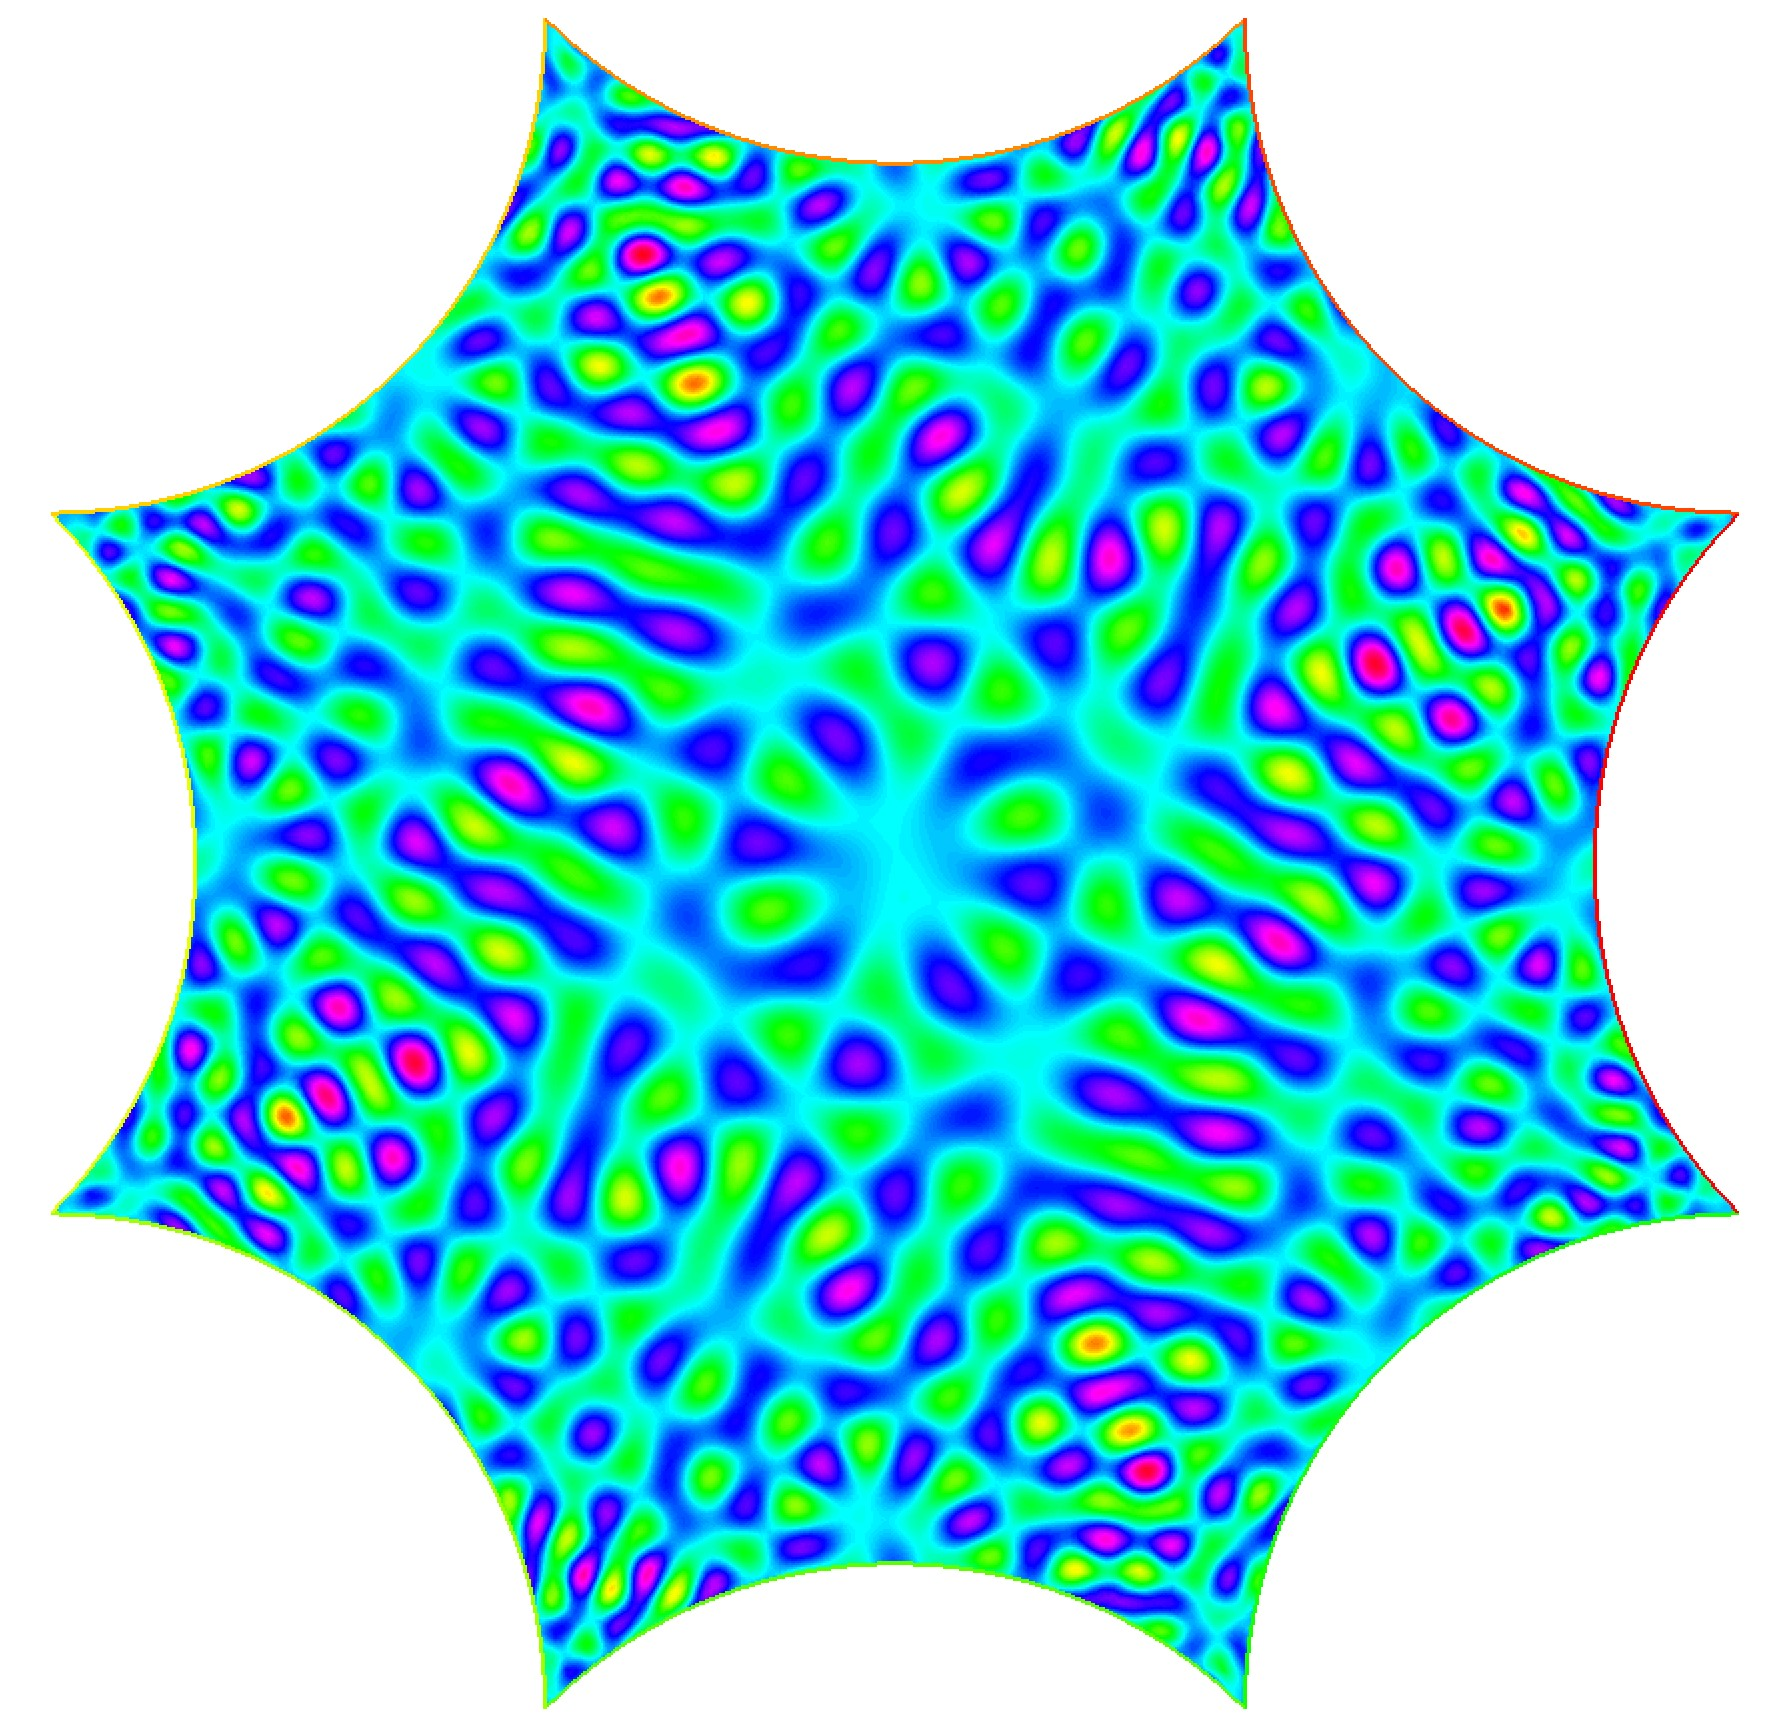
\includegraphics[scale=0.08,angle=0]{bolza8.jpg}
    %\caption{Variabili $X_{n}$}
    \label{fig:eig_bolza7}
  \end{subfigure}
  \noindent\\
  \decoRule
  \caption{Bolza surface is an arithmetic hyperbolic surface, thus eigenfunctions equidistributes on the surface.}
  \label{fig:bolza_eig_equidistr}
\end{figure}



\begin{figure}[H]
\centering
  \begin{subfigure}[b]{0.4\textwidth}
  \centering
    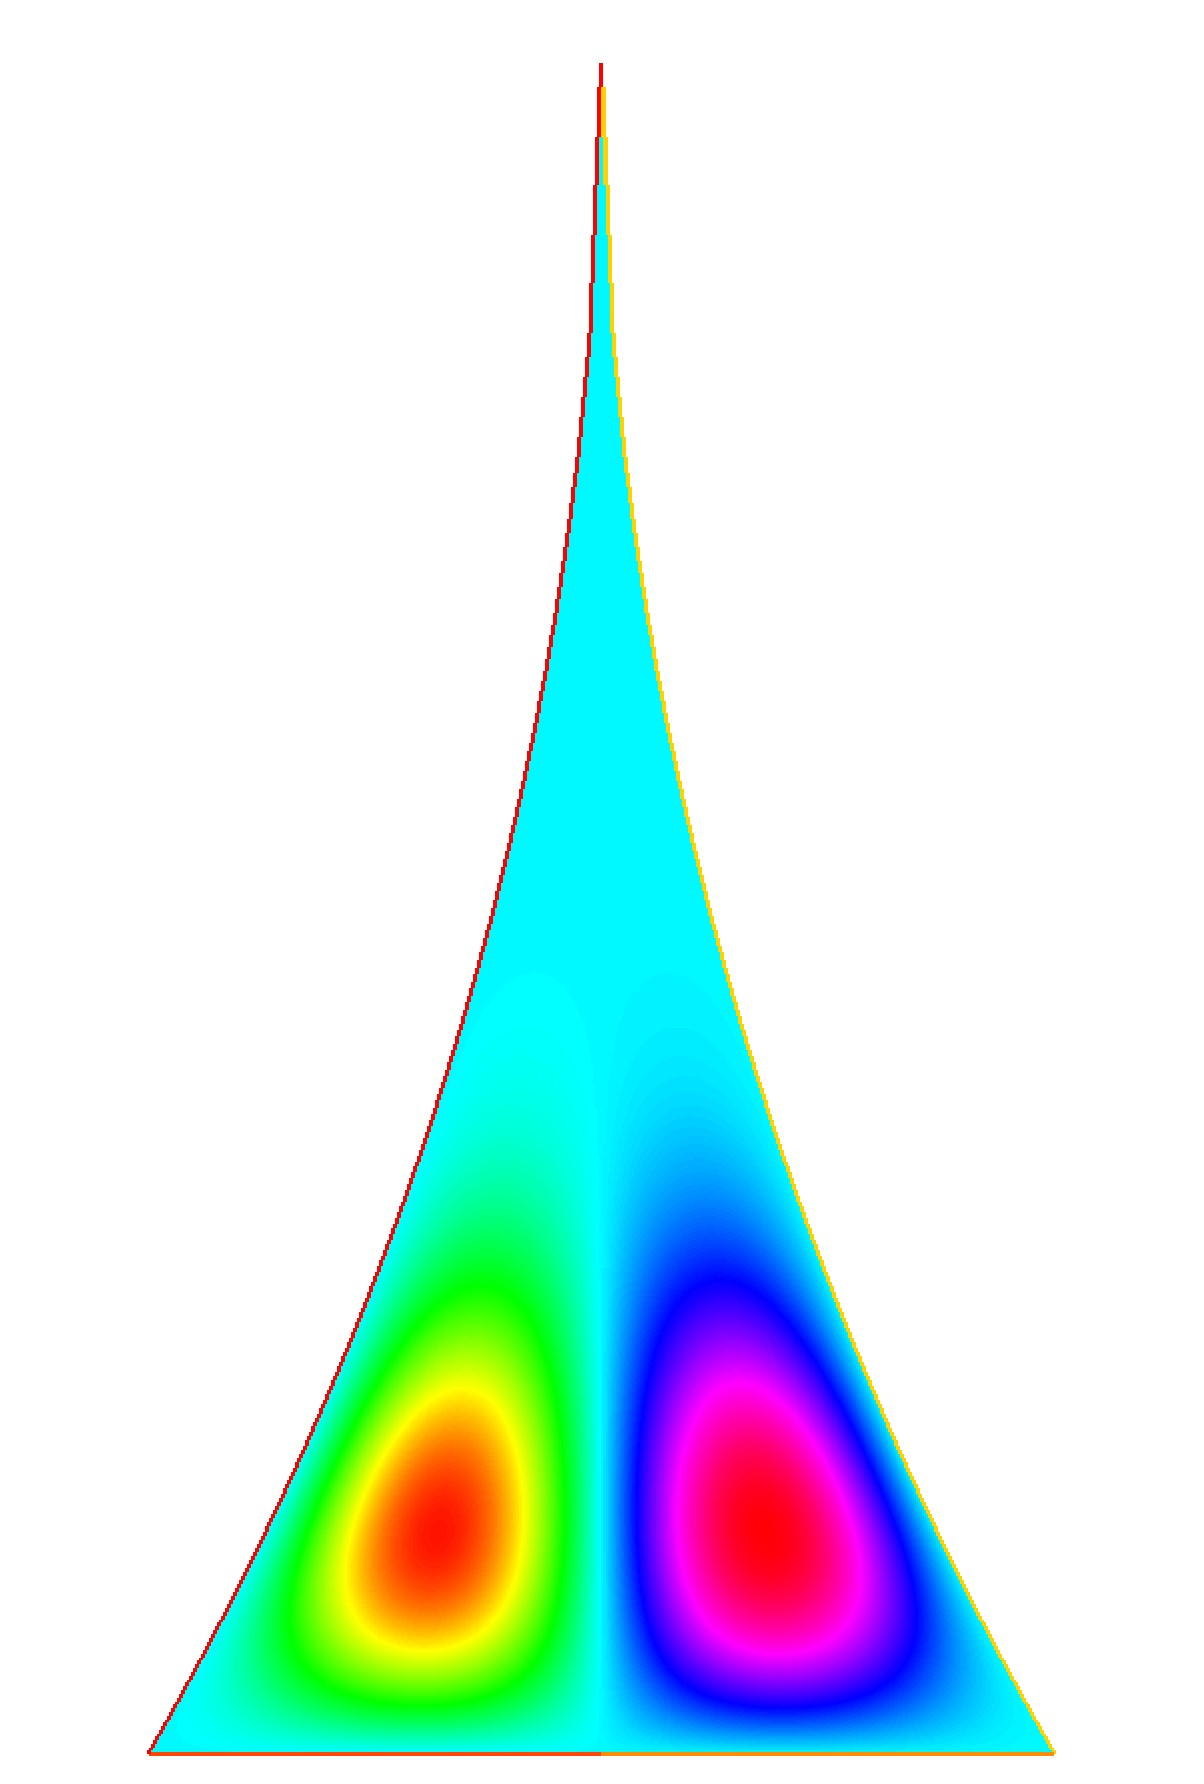
\includegraphics[scale=0.15,angle=0]{modular1.jpg}
    %\caption{Variabili $X_{n}$}
    \label{fig:modular_eig1}
  \end{subfigure}
  %
  \begin{subfigure}[b]{0.4\textwidth}
  \centering
    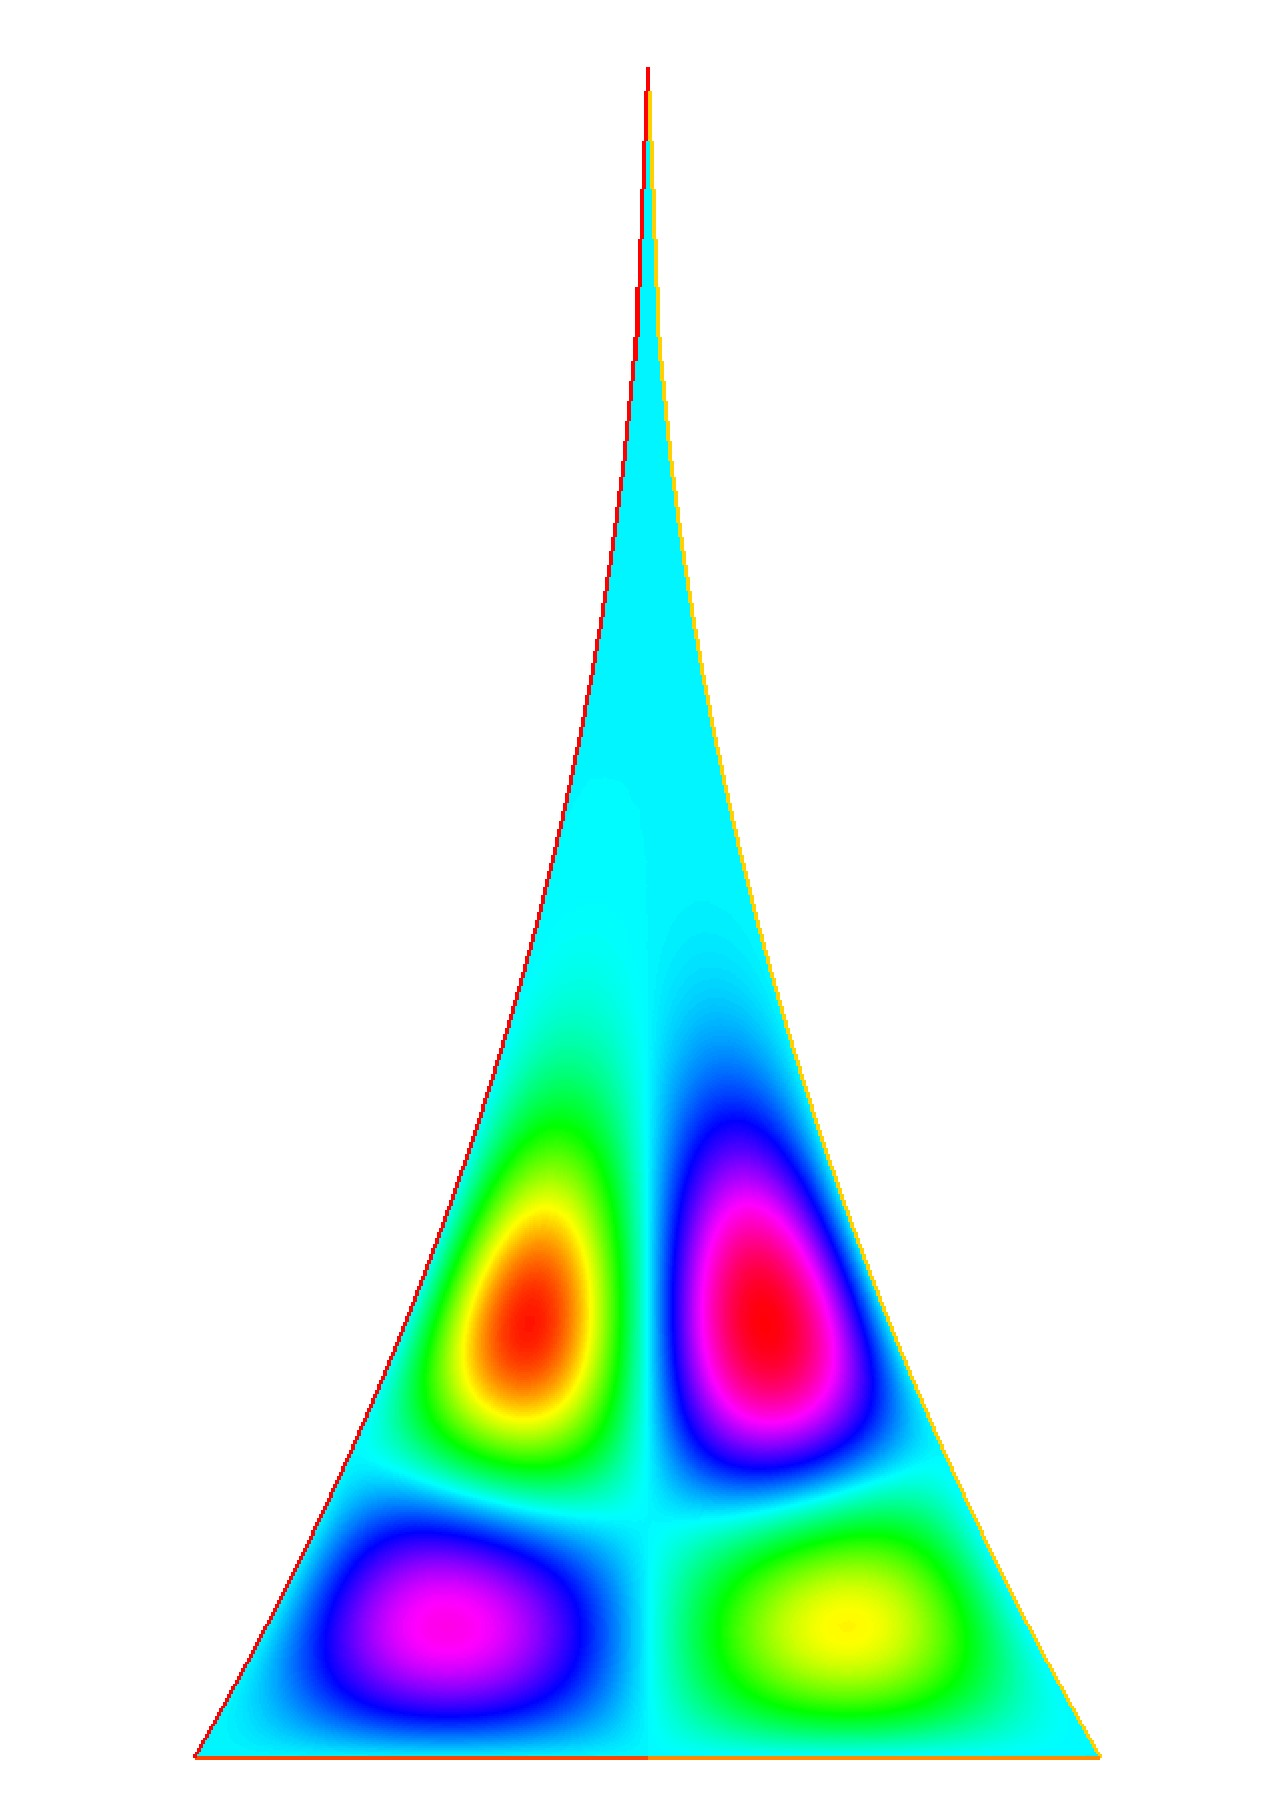
\includegraphics[scale=0.15,angle=0]{modular3.jpg}
    %\caption{Variabili $X_{n}$}
    \label{fig:modular_eig2}
  \end{subfigure}
  \noindent\\
  \decoRule
  \caption{The first two eigenfunctions of the modular surface, see on the Poincaré disk model $\Disk$. The corrisponding eigenvalues are $\lambda_{1}=91.12\ldots$ and $\lambda_{2}=148.43\ldots$, see \cite{Sarnak:review}.}
  \label{fig:first_two_eig_modular}
\end{figure}



METTI  ALTRE FIGURE EIGENFUNCTIONS FATTE DA TE 


\subsection{Numerical methods}

The first attempts to investigate the spectrum of the modular surface $X(1)$ were carried out in \cite{Cart:comput}. After those not-so-successfully attemps, other simulations were made and, among the eigenvalues $1/4+t^{2}=\lambda$, some Riemann zeros $1/2+\imi t$ suddenly appeared. The reason was later discovered by Hejhal \cite{Hejhal:triang}, who also developed a useful (heuristic) method to compute spectra of modular surfaces, and later improved by the already mentioned Friderik Stromberg, in his PhD thesis.\\

The reason behind the presence of Riemann zeta's zeros was the following: the numerical methods used until then were faulty in allowing the eigenfunctions to have logarithmic singularities. Obviously, these were not real eigenfunctions. The method developed by Heijal is now known as \virg{collocation}. The eigenfunctions, i.e. cusp forms, considered have a Fourier expansion in $z=x+\imi y$ given by 
\[
\vphi^{+}(z)=\sum_{n=1}^{\infty}\rho_{\vphi}(n)y^{1/2} K_{\imi t_{\vphi}}(2\pi ny)\cos(2\pi nx)
\]
and
\[
\vphi^{-}(z)=\sum_{n=1}^{\infty}\rho_{\vphi}(n)y^{1/2} K_{\imi t_{\vphi}}(2\pi ny)\sin(2\pi nx)
\]
where $\vphi^{\pm}(z)$ are, respectively, even and odd eigenfunctions respect to the vertical axis $\Re(z)=0$ (see \cite{Stark:mod_forms},\cite{Sarnak:review} for details) and the eigenvalue is $\lambda=1/4+t^{2}_{\vphi}$.\\
The unknowns in these expressions are the coefficients $\rho_{\vphi}(n)$ and the eigenvalue parameter $t_{\vphi}$. We will roughly described a main method un this subject, due to Heijal, which is suited for \virg{not-so-big} eigenvalue parameters $t_{\vphi}$, but there are other modern methods, due to Stark, Barnett, Stromberg and Strohmaier among the others, which cover different cases.\\

The Bessel function $K_{\imi t_{\vphi}}(y)$ is exponentially decreasing for $y\gg\abs{t_{\vphi}}$, so that the series expressing $\vphi^{\pm}$ is approximated with an accurancy of $O(\e^{-2\pi M})$ for $y\geq\frac{\sqrt{3}}{2}$, when both series are truncated at $n=M$. The functions $\vphi(z)$ are already $1$-periodic\footnote{The eigenfunctions have to be $\PSL_{2}\Z$-invariant and $\PSL_{2}\Z=\spn{J,S}$, where $Jz=-1/z$ and $Sz=z+1$, see section \ref{subsec:hyp_surfc}.} so what is missing is the $J$-invariance, i.e. the condition $\vphi(-1/z)=\vphi(z)$.\\
This method is \virg{good} to get eigenvalues of $X(1)$ such that $\lambda\lesssim 250000$. At first, truncate the series at $n=M$ and choose evenly distributed points $z_{1},\ldots,z_{M}\in D_{2\imi}$ ($z_{i}=x_{i}+\imi y_{i}$), where $D_{2\imi}$ is the Dirichlet fundamental domain of $X(1)$ with center $2\imi$. The condition $\vphi(-1/z)=\vphi(z)$ for the truncated series $\vphi^{(M)}(z)$ and the chosen sample gives the system of equations
\[
\vphi^{(M)}(z_{j})=\vphi^{(M)}(-1/z_{j}),\forall i=1,\ldots, M
\] 
which is a homogeneous linear system of $M$ equations with $M$ unknowns. Each equation is of the form
\[
\sum_{n=1}^{M}\rho(n)A_{n,j}(t)=0
\]
where\footnote{We consider the even case for $\vphi$.}
\[
A_{n,j}(t)=A_{n}(z_{j},t)\coloneqq\sqrt{Jy_{j}}K_{\imi t}(2\pi n Jy_{j})\cos(2\pi nJx_{j})-\sqrt{y_{j}}K_{\imi t}(2\pi n y_{j})\cos(2\pi nx_{j}).
\]
One way to go on, at this point, is to seek solutions $t\leq T$ of the equation 
\[
\det A(t)=0
\]
where $A$ is the matrix obtained by elements $A_{n,j}(t)$. However, to speed up the process it is more convenient to choose a second set of points $w_{2},\ldots,w_{M}$ and to solve the double system of equation (setting $\rho(1)=1$)
\begin{equation}
\label{eq:system_heijal_eq}
\begin{cases}
\sum_{n=2}^{M}\rho^{(z)}(n)A_{n}(z_{j},t)&-A_{1}(z_{j},t)\\
\sum_{n=2}^{M}\rho^{(z)}(n)A_{n}(w_{j},t)&-A_{1}(w_{j},t)
\end{cases}
,\quad\forall j=2,\ldots,M.
\end{equation}

For a true eigenvalue parameter $t_{\vphi}$ it should hold
\[
\rho^{(z)}(n)=\rho^{(w)}(n),\quad \forall n=2,\ldots,M.
\]
but it is not granted for approximated values $t$. Hence one chooses the $t$'s for which this condition holds. This works well until $T\simeq 500$, but after this points the system \eqref{eq:system_heijal_eq} becomes ill conditioned.


\section{Spectral statistics and Random Matrix Theory}

In order to tackle the problem, without getting involved in complications to the geometrical constrainst (symmetry groups, different metric and so and so forth), this field has encoutered the method of \emph{\textsc{spectral statistics}}.\\
In this case, the approach is exactly the contrary: obtaining geometrical informations from the spectra of the Laplacian, with tools from, for example, the Random Matrix Theory \RMT. In particular, getting analyitical informations about the spectra of the Laplacian is an hopeless task, but nonetheless it is possible to get asymptotical informations, starting from statistical knowledge of the corrispondent classical underlying billiard. In this sense, Weyl's law is a good example, as it lets to recover the area of the domain, from the distribution of the eigenvalues.\\
For this reason (distribution of the eigenvalues) the \emph{Nearest Neigbour Spacing Distribution} is introduced: it a function that counts the fraction of eigenvalues $\lambda_{n}$ less than a fixed real $\lambda$, which are distant from the next eigenvalue $\lambda_{n+1}$ at most $s$. In other words, the expression of the \NNSD is 
\[
P(s,N)\coloneqq\frac{1}{N}\sum_{j=1}^{N}\one_{\{s>\lambda_{n+1}-\lambda_{n}\}}.
\]
In general, the sequence $\lambda_{n}$ is sufficiently randomized, so it \virg{should exist} a limit distribution $p(s)=\lim_{N\to\infty}P(s,N)$ so that
\[
\lim_{N\to\infty}\int_{0}^{\infty}p(s,N)h(s)\dd s=\int_{0}^{\infty}p(s)h(s)\dd s
\]
for a smooth function $h$ with compact support. In this context, we can find the true starting point of the modern Quantum Chaos, which is the \emph{Berry-Tabor conjecture}.

\begin{impConj}{Berry-Tabor,1977}{}
For \virg{generic integrable systems} the limit distributions $P(s)$ of the \NNSD  is equal to the waiting time distribution coincides with the corresponding quantity for
a sequence of uncorrelated levels (the Poisson ensemble), i.e. the waiting time distribution of a Poisson process: $p(s)=c\e^{-cs}$, with $c=\Area/4\pi$.
\end{impConj}

Another dramatic insight about the possible forms of the quantity $p(s)$ is given by the following conjecture, regarding the chaotic, ergodic case.

\begin{impConj}{Bohigas, Giannoni, and Schmit, 1984}{BGS}
If the underlying classical dynamics is ergodic, then $p(s)$ coincides with the corrisponding quantity for the eigenvalues of a suitable ensemble of \emph{random matrices}.
\end{impConj}


Until now the conjecture has not been proved in its generality. However, there is a vast list of
numerical studies based on a wide variety of systems that support its validity; of particular interest are, of course, hyperbolic dynamical systems arising from arithmetical groups (like the modular surface and the bolza surface) and an exstensive analysis is developed in \cite{bogomolnyaltri:article} and \cite{bogomolny:article}, a work by Bogolmy, Bohigas, Giannoni, and Schmit which gives this thesis title. 
\begin{remark}
\label{remark:zeta_spectra}
It is a curious thing, object of undergoing studies, that the statistics of conjecture \ref{impConj:BGS} is similar to the distribution of the zeros of Riemann's zeta function $\zeta(z)$. 
\end{remark}

A mathematically rigorous formulation of the now-so-called Random Matrix Theory \RMT was established by Freeman Dyson in a series of papers. He introduced the classification of the Gaussian random matrix ensembles according to their invariance properties under time reversal. In particular, he proved the existence of only three classes for such matrices. He said:\\
\textit{
What is here requiered is a new kind of statistical mechanics, in which we renounce exact knowledge not of the state of the
system but of the system itself. We picture a complex nucleus as a \virg{black box} in which a large number of particles are interacting according to unknown laws. The problem then is to define in a mathematically precise way an ensemble of systems in which all possible laws of interaction are equally possible
.}\\
\hspace*{10cm}-\emph{Freeman Dyson}\\
\noindent\\

\begin{defin}[Gaussian Random Matrix]
\label{def:gauss_rand_matrix}
The Gaussian random matrix $H$ is a matrix from an ensemble of matrices with probability distribution $P(H)$, such that
\begin{compactitem}
\item the probability distribution have to be invariant under a prescribed transformations $W$, $P(H)=P(W^{-1}HW)$;
\item matrix elements of $H$ are statistically indipendent.
\end{compactitem}
\end{defin}

The possible Gaussian random matrix ensembles are then:
\begin{compactitem}[1)]
\item \textbf{Gaussian Orthogonal Ensemble} \GOE : related to time-reversal systems, this ensemble is invariant under orthogonal trasformations. The matrix $H$ mirroring the Hamiltonian of the system is real symmetric and has $N(N+1)/2$ indipendent real components.   
\item \textbf{Gaussian Unitary Ensemble} \GUE : related to  non time-reversal systems, this ensemble is invariant under unitary trasformations. The matrix $H$ mirroring the Hamiltonian of the system is complex Hermitian and has $N^{2}$ indipendent real components.
\item \textbf{Gaussian Symplectic Ensemble} \GSE : related to time-reversal systems with particular features, this ensemble is invariant under symplectic trasformations. The matrix $H$ mirroring the Hamiltonian of the system is quaternionic Hermitian and has $N(2N-1)$ indipendent components. This ensample is used only for very particular systems.
\end{compactitem}

After suitable normalization, the \NNSD for the three Gaussian ensembles are gives by:
\begin{compactitem}
\item \GOE: $p(s)=\frac{\pi}{2}\exp\left(-\frac{\pi}{4}s^{2}\right)$;
\item \GUE: $p(s)=\frac{32}{\pi^{2}}s^{2}\exp\left(-\frac{4}{\pi}s^{2}\right)$;
\item \GSE: $p(s)=\left(\frac{64}{9\pi}\right)^{3}s^{4}\exp\left(-\frac{64}{9\pi}s^{2}\right)$.
\end{compactitem}

\begin{figure}[H]
\centering

    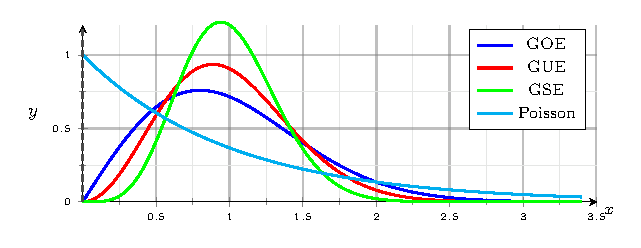
\includegraphics[scale=1,angle=0]{distributions.pdf}
    %\caption{Variabili $X_{n}$}

  %
  \noindent\\

  \decoRule
  \caption{Different distributions from Random Matrix Theory.}
  \label{fig:different_distributions}
\end{figure}


Quite remarkably, the distribution eigenvalues on the modular surface $X(1)=\PSL_{2}\Z$ follows a Poisson distribution (\cite{Rudnick:whatIs}).


\begin{figure}[H]
\centering

    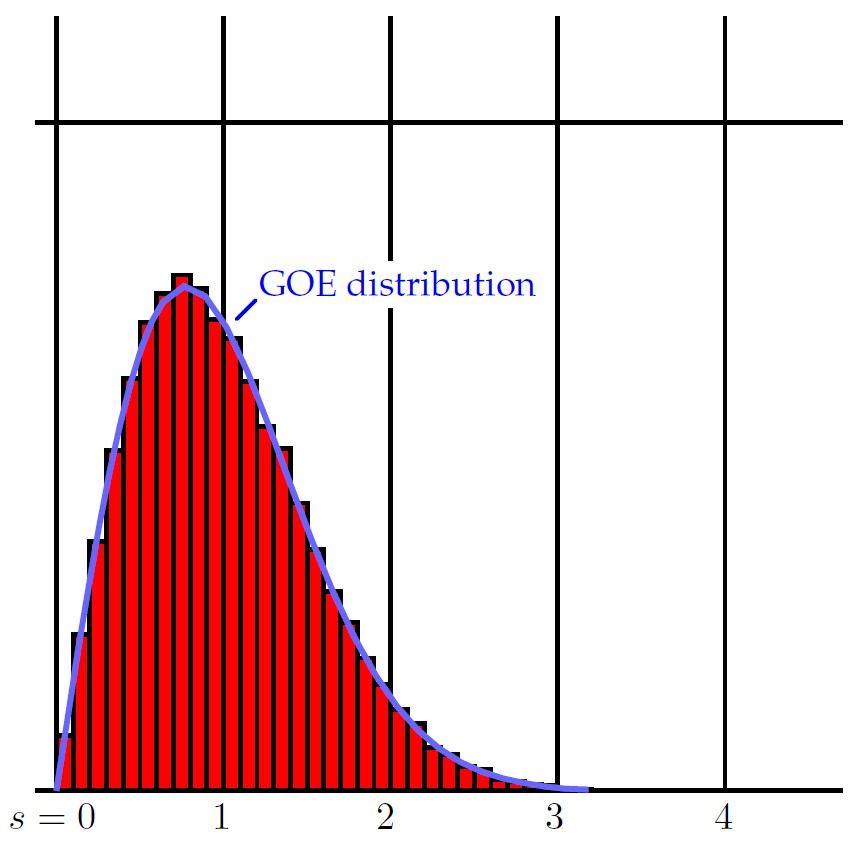
\includegraphics[scale=0.5,angle=0]{goe.jpg}
    %\caption{Variabili $X_{n}$}

  %
  \noindent\\

  \decoRule
  \caption{From \cite{Rudnick:whatIs}. Normalized gaps
between roughly 50000 sorted eigenvalues
for the Barnett's stadium \ref{fig:barnett_eigenfunction}. The distributions follows the \GOE distribution.}
  \label{fig:goe_distrib}
\end{figure}


On the contrary, the distribution is expected, by enormous numerical simulations by Odlyzko \cite{Odly:comput}, to follow the rare \GUE distribution (\cite{Rudnick:whatIs}).


\begin{figure}[H]
\centering

    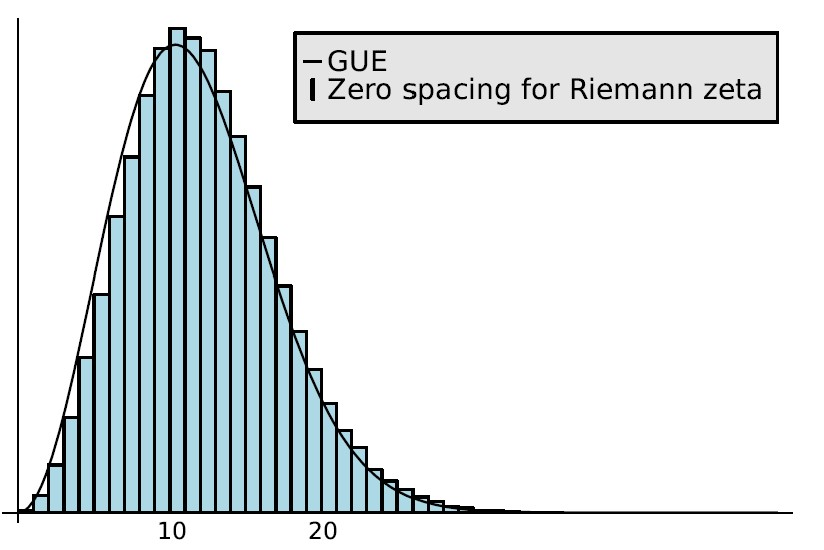
\includegraphics[scale=0.55,angle=0]{zeros_zeta_gue.jpg}
    %\caption{Variabili $X_{n}$}

  %
  \noindent\\

  \decoRule
  \caption{From \cite{Rudnick:whatIs}, computations by \cite{Odly:comput}. Distributions of zeros of Riemann zeta function.}
  \label{fig:gue_distrib_zeta}
\end{figure}



For further details, we refer to CITA. The hope of this approach is to increase the understanding about how integrable and chaotic systems differ in the semiclassical limit.










%----------------------------------------------------------------------------------------
%	SECTION 1
%----------------------------------------------------------------------------------------



\section{Conclusion}

To be done




\subsection{Billiard and spectral simulations}



